\chapter{Técnicas e Decisões de Design}

Neste presente capitulo serão explorados os conceitos de design aplicados no projeto
desenvolvido assim como as decisões tomadas durante o processo de desenvolvimento. 
O design do jogo é um elemento crucial para garantir uma experiência envolvente e 
satisfatória para os jogadores, envolve a criação de mecânicas com técnicas de design,
complementa o projeto como um todo.

Serão apresentados métodos científicos e técnicos utilizados para a construção do jogo, 
bem como as escolhas pessoais e criativas que influenciaram o desenvolvimento do projeto. 
O objetivo é estabelecer uma compreensão clara do processo de design e das decisões tomadas.

\section{Técnicas utilizadas}

Nas subsecção consequentes serão descritas e apresentadas as técnicas de design utilizadas no desenvolvimento do projeto,
incluindo a aplicação de princípios de design e metodologias de desenvolvimento.

\subsection{\textit{Framework} MDA (\textit{Mechanics, Dynamics, Aesthetics})}

O \textit{framework} MDA, desenvolvido por \textcite{framework-mda}, é uma abordagem amplamente 
utilizada no design de jogos concentrados em três componentes 
principais: Mecânicas, Dinâmicas e Estéticas.
As Mecânicas referem-se às regras e sistemas que governam o jogo, 
as Dinâmicas são as interações inerentes entre as mecânicas e os jogadores, 
e as Estéticas são as emoções e experiências que os jogadores vivenciam ao jogar.

Posto isto, o \textit{framework} MDA foi utilizado como guia para a construção do jogo,
e o diagrama apresentado na Figura \ref{MDA_Diagram} ilustra a relação entre as mecânicas, dinâmicas e estéticas do jogo desenvolvido.

\begin{figure}[h!]
    \centering
    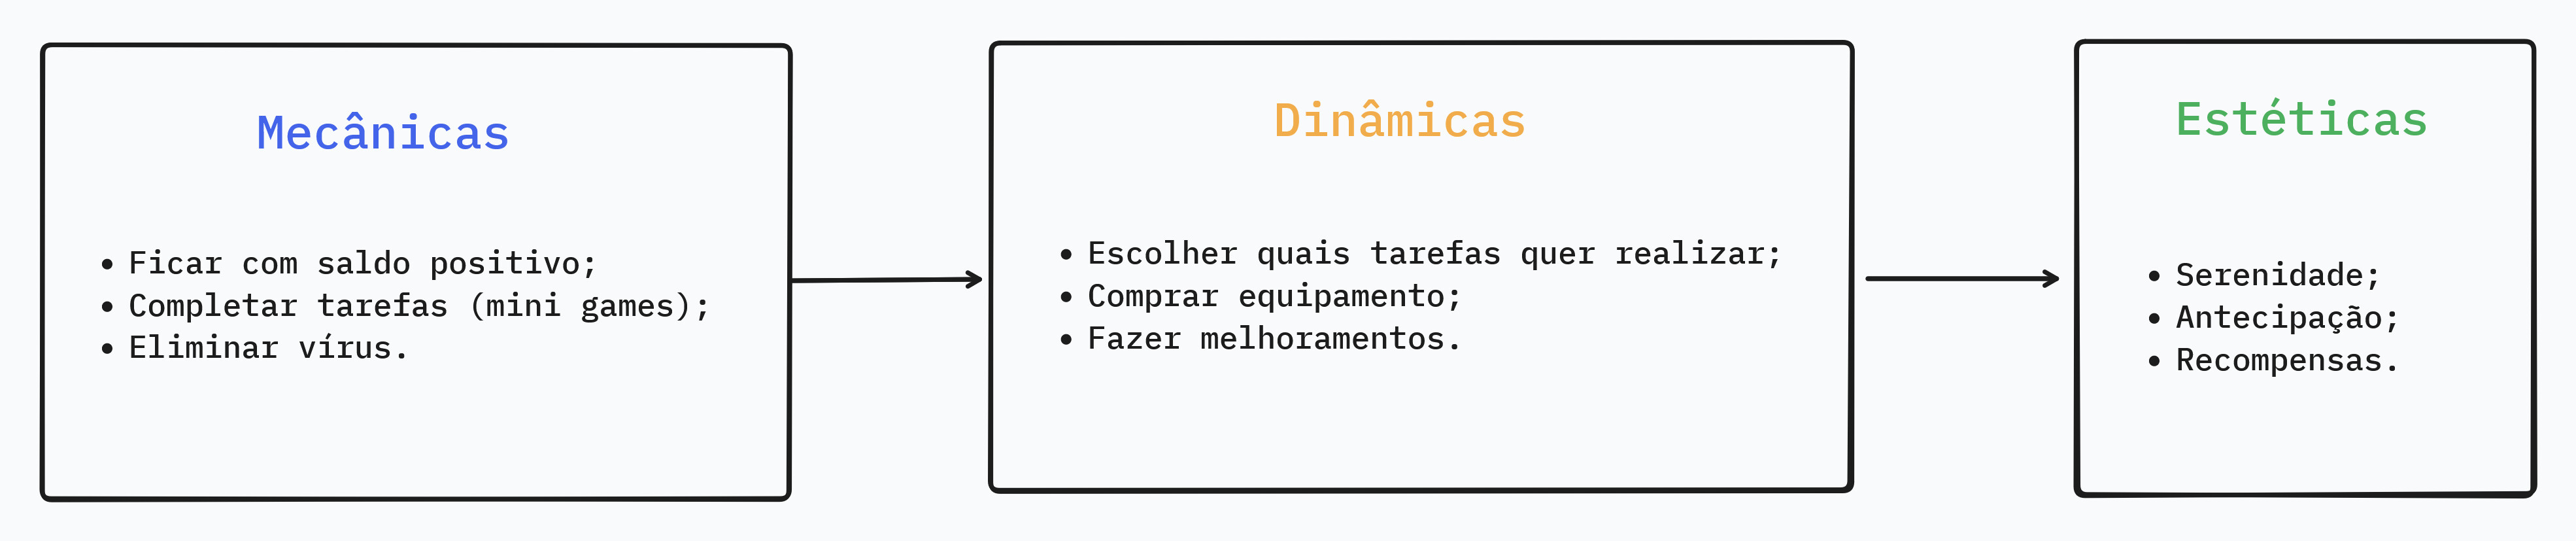
\includegraphics[width=1\textwidth]{Diagramas/MDA.jpg}
    \caption{Diagrama do \textit{framework} MDA aplicado ao jogo desenvolvido.}
    \label{MDA_Diagram}
\end{figure}

\subsection{\textit{Flow}}


Embora venha da psicologia, o trabalho de \textcite{flow} é a base para o design de 
progressão em jogos. Define o equilíbrio entre a dificuldade do desafio e a habilidade do jogador para evitar o tédio ou a ansiedade.
O conceito de \textit{Flow} foi aplicado no design do jogo para garantir que os 
jogadores se mantenham engajados e motivados a continuar jogando, 
proporcionando desafios adequados ao nível de habilidade dos jogadores.

Na Figura \ref{Flow_Diagram} é possível observar um diagrama que ilustra o conceito de \textit{Flow} aplicado ao design do jogo.

\begin{figure}[h!]
    \centering
    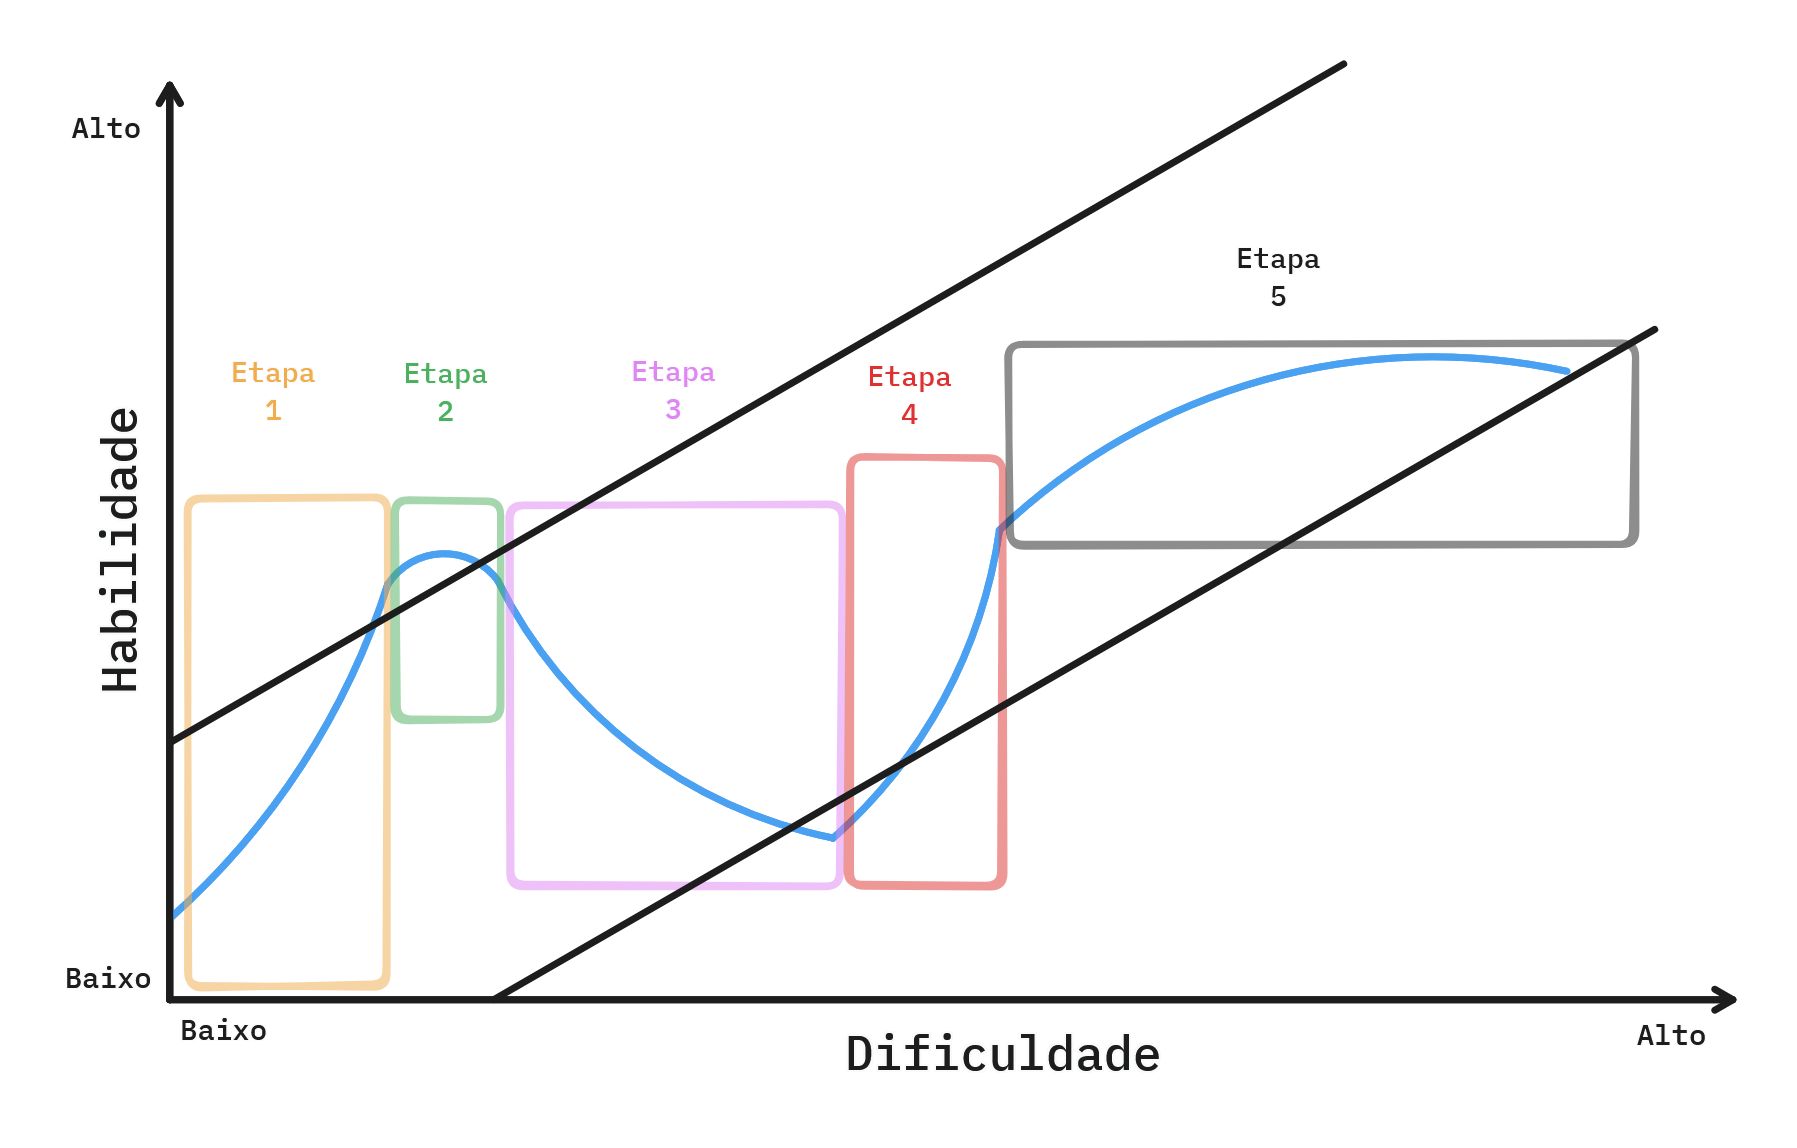
\includegraphics[width=0.5\textwidth]{Diagramas/Flow Graph.png}
    \caption{Diagrama do conceito de \textit{Flow} aplicado ao design do jogo.}
    \label{Flow_Diagram}
\end{figure}

O diagrama é divido em 5 etapas, onde cada uma dela representam momentos específicos do jogo.
A 1º etapa representa os primeiros momentos do jogo, onde o jogador está a aprender as mecânicas básicas
e a preceber o que tem de fazer para progredir, como tal é representa por uma curva crescente.

A 2º etapa é caracterizada pela adptação do jogador às mecânicas introduzidas na etapa anterior,
como tal a curva de \textit{flow} começa a descer, uma vez que devida a adaptação do jogador, o desafio se torna mais fácil.

A 3º etapa representa a habituação do jogador às mecânicas, assim como a repetição de desafios semelhantes,
o que leva a uma curva de \textit{flow} com um declive negativo, uma vez que o jogador começa
a sentir-se entediado e desmotivado a continuar jogando.

A 4º etapa, por contraste com a anterior, é caracterizada pela introdução de inimigos, o que indiretamente implica a introção de
mecânicas novas e quebra o ciclo até aquele momento, o que leva a um aumento da dificuldade percebila pelo
jogador, o que indiretamente justifica o aumento do \textit{flow}.

Por fim a 5º etapa é caracterizada por uma adaptação, da parte do jogador, às
mecânicas introduzidas na etapa anterior, com as mecânicas iniciais,
o que resulta numa curva de \textit{flow} com um crescimento bastante moderado, uma vez que o
jogador já tem uma base sólida construida com as mecânicas anteriores, 
o que o torna a \textit{gameplay} muito mais previsível, resultando assim numa 
curva de \textit{flow} mais estável e menos propensa a declives acentuados.

Em suma, a progressão do jogo utiliza a alternância entre a introdução de novos 
desafios e períodos de adaptação para modular a experiência do utilizador. Ao gerir 
estas cinco etapas, o design garante que o jogador no estado de \textit{Flow}, 
equilibrando a curva de aprendizagem com momentos de novidade, assegurando assim uma 
experiência envolvente, fluida e recompensadora do início ao fim.

\subsection{Modelo de \textit{Hook}}

No âmbito do game design contemporâneo e do desenvolvimento de produtos digitais, a 
retenção de utilizadores tornou-se um dos indicadores de desempenho mais críticos. 
Neste contexto, o Modelo de Hook \textit{(Hook Model)}, conceptualizado por \textcite{modelo_hook}, 
surge como uma estrutura teórica e prática desenhada para fomentar a criação de 
hábitos através da interação contínua com o produto.

Ao contrário de abordagens baseadas meramente em publicidade agressiva, o Modelo de 
Hook foca-se na psicologia do utilizador, ligando os seus problemas e necessidades 
quotidianas a uma solução tecnológica específica. Este modelo é composto por um ciclo 
iterativo de quatro fases fundamentais: o Gatilho \textit{(Trigger)}, a Ação \textit{(Action)}, a 
Recompensa Variável \textit{(Variable Reward)} e o Investimento \textit{(Investment)}.

Posto isto, o Modelo de Hook utilizado no desenvolvimento deste projeto, é caracterizado
pelos seguintes elementos:

\begin{itemize}
    \item \textit{Trigger}: Curiosidade pela temática do jogo, apelo pelo visual e apelo de curiosidade pelo uso de técnicas e tecnologias reais, senso de colecionismo. Retornar ao jogo para obter o dinheiro que está em estado pendente.
    \item \textit{Ação}: Resolução de puzzles rápidos, cerca de 60 segundos, sobre a forma de \textit{minigames}, otimização de recursos e processos. Derrotar inimigos e fazer melhoramentos gerais.
    \item \textit{Recompensas}: Obtenção de novos recursos, equipamentos e troféus, (colecionismo), melhoramento de equipamentos.
    \item \textit{Investimento}: Investimento de tempo e esforço para a progressão no jogo.
\end{itemize}

Alguns elementos presente no modelo assim, como troféus e melhoramento de equipamentos (tanto 
de servidores como de armas), estão presente no conceito de design do jogo, no entanto,
não estão contenplados no projeto desenvolvido, uma vez que não eram o foco principal e
não existiu tempo suficiente para a sua implementação.

\section{Decisões de Design}

\subsection{\ac{UI} e referências técnicas}

A \textit{User Interface} (\ac{UI}) do jogo está presente durante toda a \textit{gameplay},
como tal construir uma \ac{UI} clara e que se enquadre no contexto do jogo, é de suma importância.
Essa visão é partilhado por \textcite{adams_fundamentals} que argumenta que a \ac{UI} deve 
atuar como uma "extensão do mundo" através do seu estilo visual.

Assim, a \ac{UI} do jogo é inspirada no estilo de programas com interfaces de \textit{Command Line Interface} (\ac{CLI}), 
com um design minimalista e funcional, utilizando cores escuras e elementos 
visuais que remetem para o contexto de Data Center, como, por exemplo, gráficos 
de barras para representar o uso de recursos, ou ícones de servidores para 
representar os equipamentos disponíveis.

\begin{figure}[H]
    \centering
    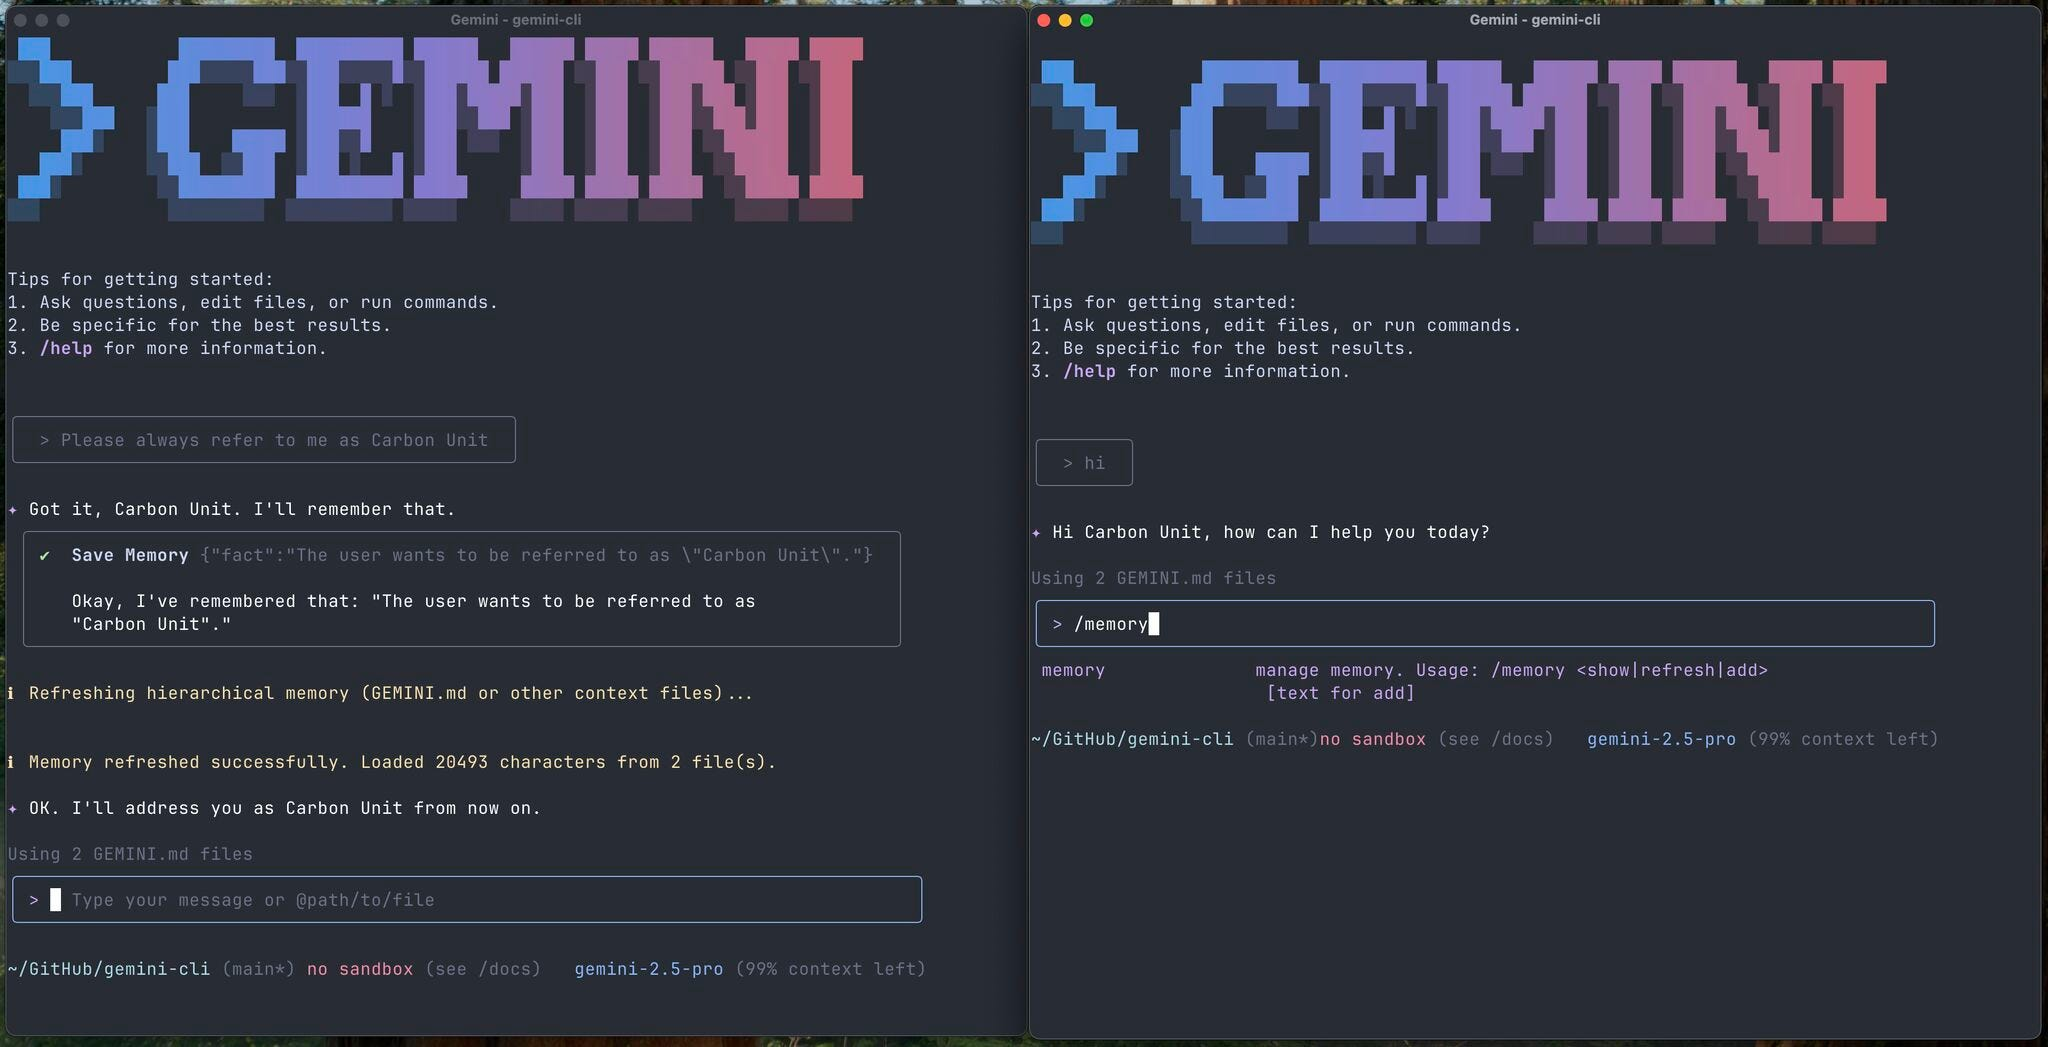
\includegraphics[width=0.8\textwidth]{images/CLI - GEMINI UI.jpg}
    \caption{Exemplo de referência - \ac{UI} do Gemini utilizado em \ac{CLI}}
    \label{UI_Gemini}
\end{figure}

\begin{figure}[H]
    \centering
    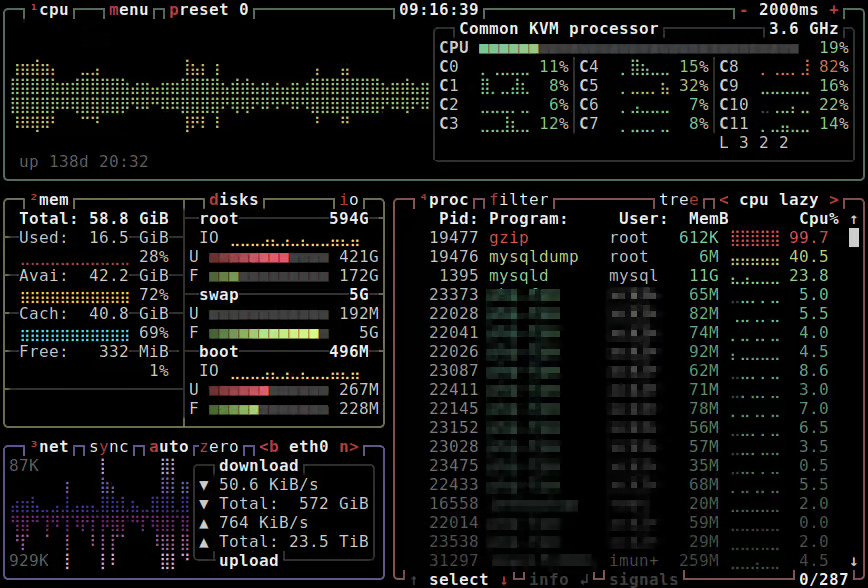
\includegraphics[width=0.8\textwidth]{images/CLI - btop UI.jpg}
    \caption{Exemplo de referência - \ac{UI} do btop}
    \label{UI_BTOP}
\end{figure}

As Figuras \ref{UI_Gemini} e \ref{UI_BTOP} apresentam exemplos de referências utilizadas 
para a construção da \ac{UI} do jogo.
A \ac{UI} das referências apresentadas é caracterizada pelo uso de cores escuras de fundo,
o uso de fonte mono espaçadas, e o uso de gráficos simples, geralmente composto, por
barras, pontos, linhas, caracteres ou quadrados.

Esses mesmos elementos podem ser visto da \ac{UI} da loja, por exemplo, (Figura \ref{Projeto_config_cpu1})
onde é utilizada uma cor de fundo escura, o uso da fonte JetBrains Mono, que é uma fonte mono espaçada,
o uso de texto e o uso de gráficos simples, como os botões e as barras de \textit{status}.

\subsection{Design de Level}

O design de level é o ato de projetar os níveis de um jogo, incluindo a 
disposição dos elementos, a criação de desafios e a definição do 
ritmo do jogo. Como tal é um dos pontos mais críticos para a construção de um jogo, uma vez
que interfere diretamente na experiência e ritmo percebido pelo jogador.

Posto isto o design de level do jogo foi desenvolvido para ser compacto,
mas que, ao mesmo tempo, cada área ofereça uma experiência distinta, que está diretamente
relacionada com a curva de \textit{flow} recebido pelo jogador.

\begin{figure}[H]
    \centering
    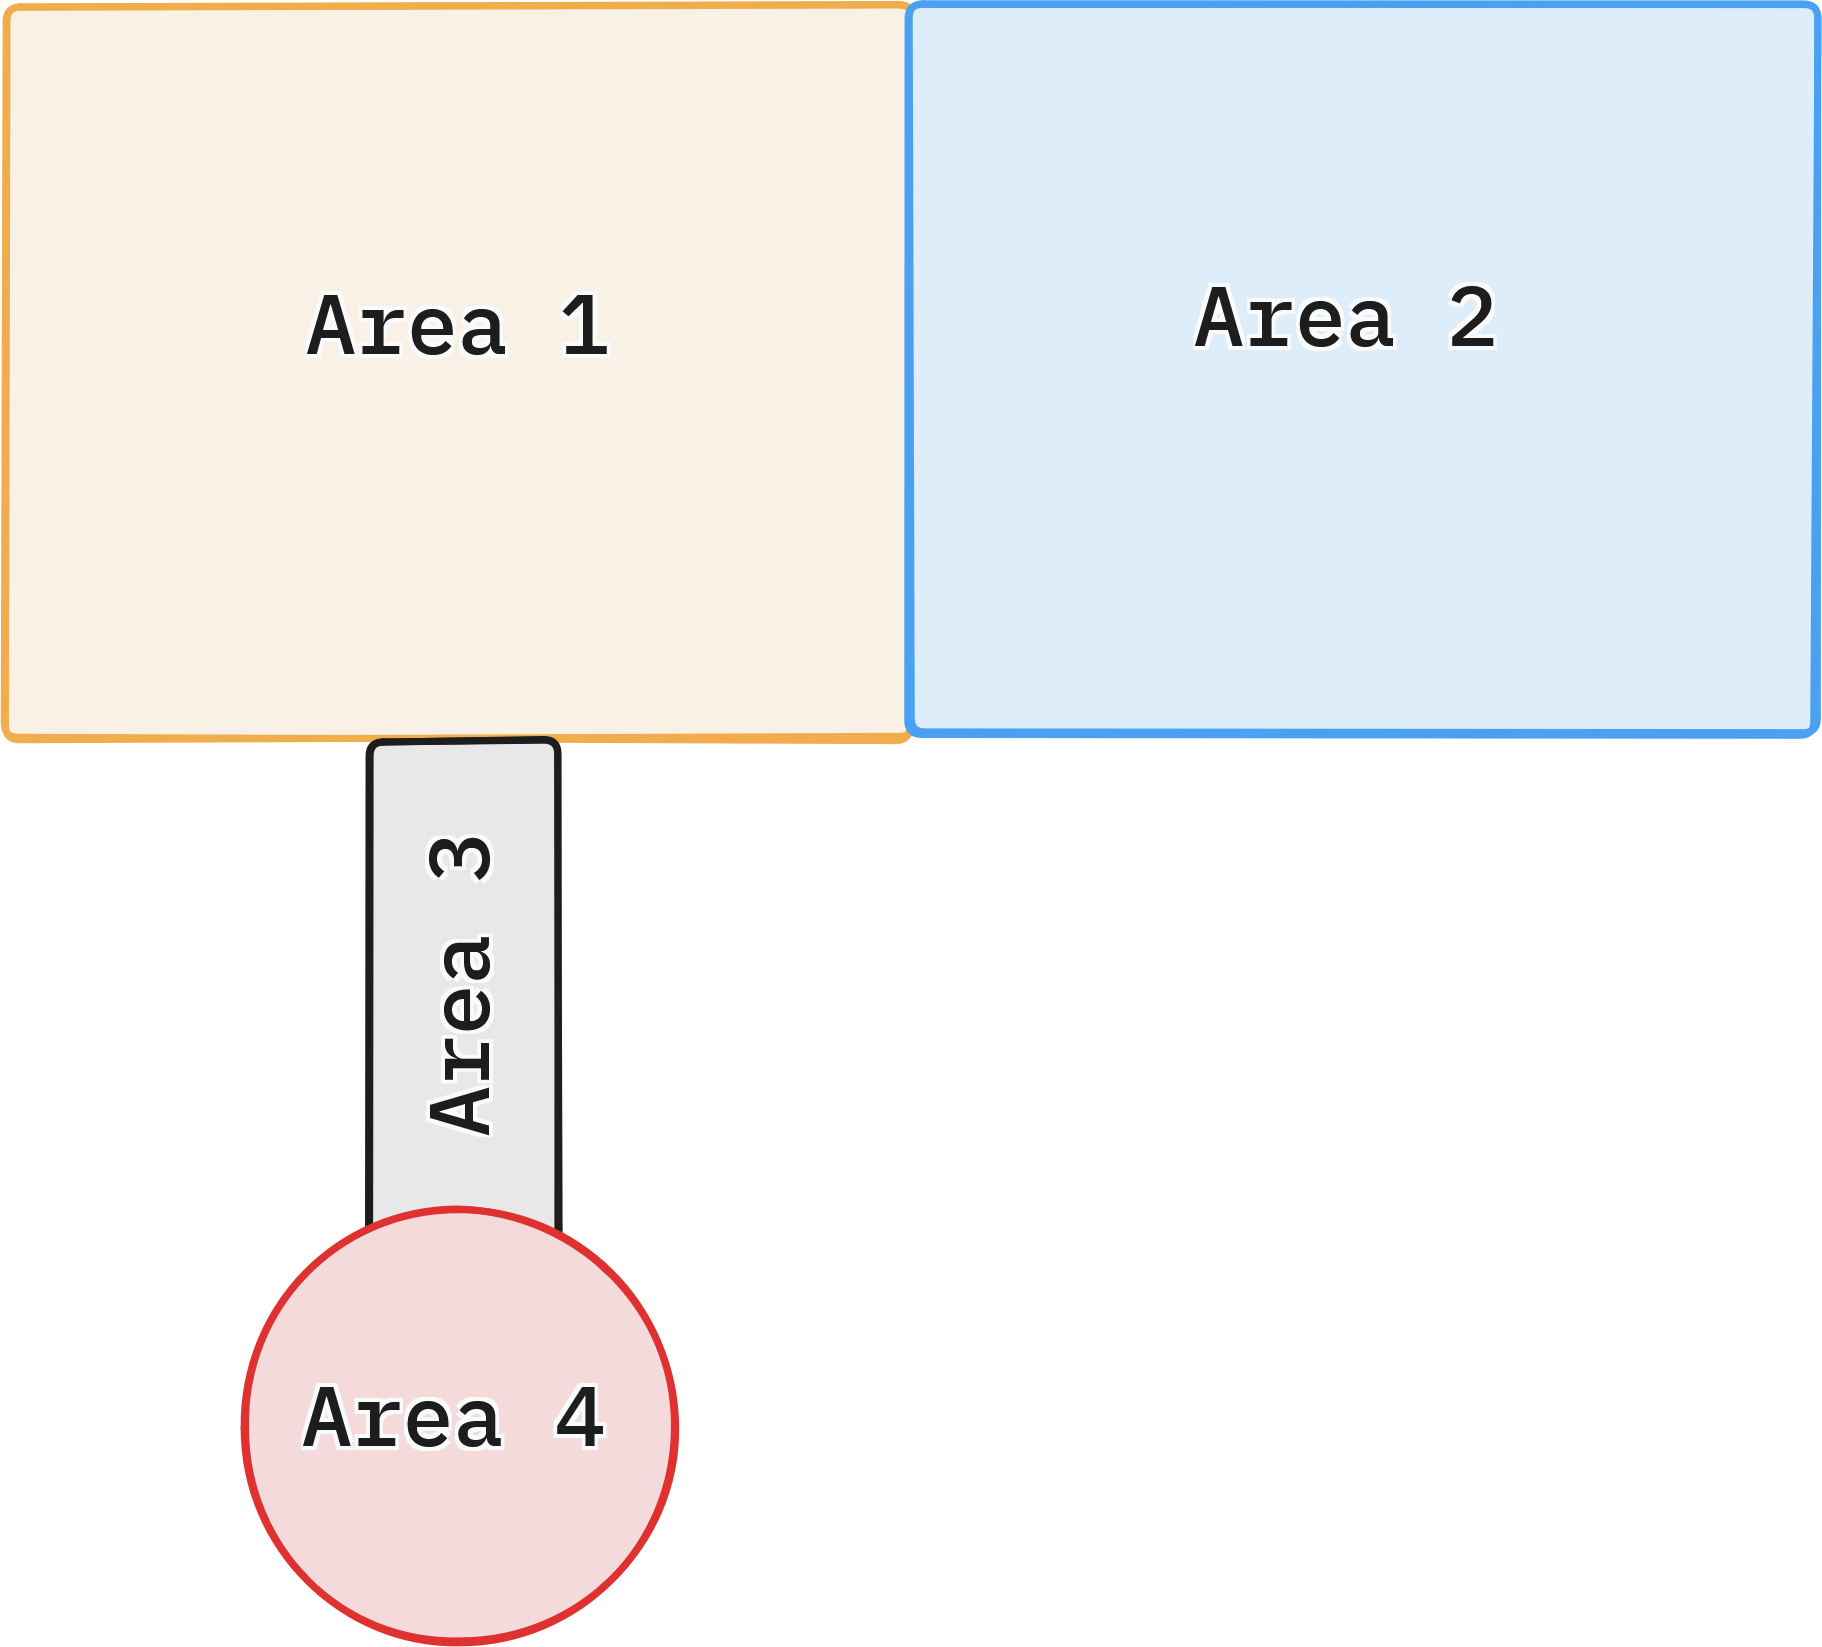
\includegraphics[width=0.8\textwidth]{Diagramas/Level Design.png}
    \caption{Level design do jogo desenvolvido.}
    \label{Level_Design}
\end{figure}

Na Figura \ref{Level_Design} está representado o design do level do jogo divido em
4 áreas distintas, sendo que cada uma tem as seguintes características:
\begin{itemize}
    \item Área 1: Área principal, onde estão localizados os servidores, e onde o jogador interage com os mesmo para resolver os puzzles, que dão dinheiro como recompensa para o jogador. É nesta área onde o jogador irá passar a maior parte do tempo, e por isso mesmo é que é a área central e a área que serve de união para as outras duas.
    \item Área 2: Área de conquista e customização, nessa área o jogador poder ver conquistas obtidas sobre a forma de troféus ou objetos de jogo. Além disso nesta área o jogador poderá interagir com o cenário para o costumizar, como por exemplo interraguir com um computador ou aparelho para fazer upgrades no cenário ou costumizar cores, etc... Esta área é caracterizada por ser um espaço de relaxamento, sem objetivos nem inimigos.
    \item Área 3: É um corredor que liga a área 1 à área 4. Não tem nenhum objetivo primário.
    \item Área 4: Área de combate, nessa área o jogador terá de utilizar de uma metralhadora para derrotar conjuntos de inimigos que irão atacar o data center. Esta área é muito especial pois é nela que existe o rompimento da \textit{gameplay}, e por isso mesmo a necessidade da existência da área 3, uma vez que o corredor representa o distânciamento do conforto proporcionado pelos puzzle da área 1. O formato geométrico dessa área também ajuda a transmitir esse contraste, uma vez que enquanto todas as outras áreas apresentam um formato quadrado, esta área apresenta um formato circular. O formato quadrado geralmente está associado a algo estável, sélido e imóvel, enquanto que o formato circular está associado a algo fluido móvel e instável. Assim, o formato circular representa a mudança de mentalidade que o jogador têm de ter, pois nessa área o jogador terá de ser rápido e capaz de desenvolver uma \textit{gameplay} dinâmica, que o combate exige. Além disso a distância geométrica entre a área 4 e área 2, é a maior de todas estando em pontas opostas, o que ajudar a transmitar a ideia de algo caótico, uma vez que a área 2 é um espaço de relaxamento.
\end{itemize}

Todavia no projeto apresentado, a área 2 não foi implementada na sua totalidade, devido a sua complexidade,
sobre tudo pela parte de desenvolvimento de troféus e pela parte de customização de cenário.

\subsection{Notificações}

Durante o desenvolvimento do jogo surgir a necessidade de desenvolver um sistema
capaz de transmitir \textit{feedbacks} informativos para o jogador. Como, por exemplo,
notificar o jogador quando é realizada com compra, completada uma tarefa, destruído um servidor, etc ...

Segundo \textcite{notificações}, o uso de notificações em jogos, é recomendável e
apresenta um efeito positivo no desempenho do jogador.

Para suprir essa necessidade foi desenvolvido um simples sistema de notificações.
O sistema envia uma notificação, sobre a forma de texto, ao jogador, sempre que acontece, alguma
das ações descritas acima.

\begin{figure}[H]
    \centering
    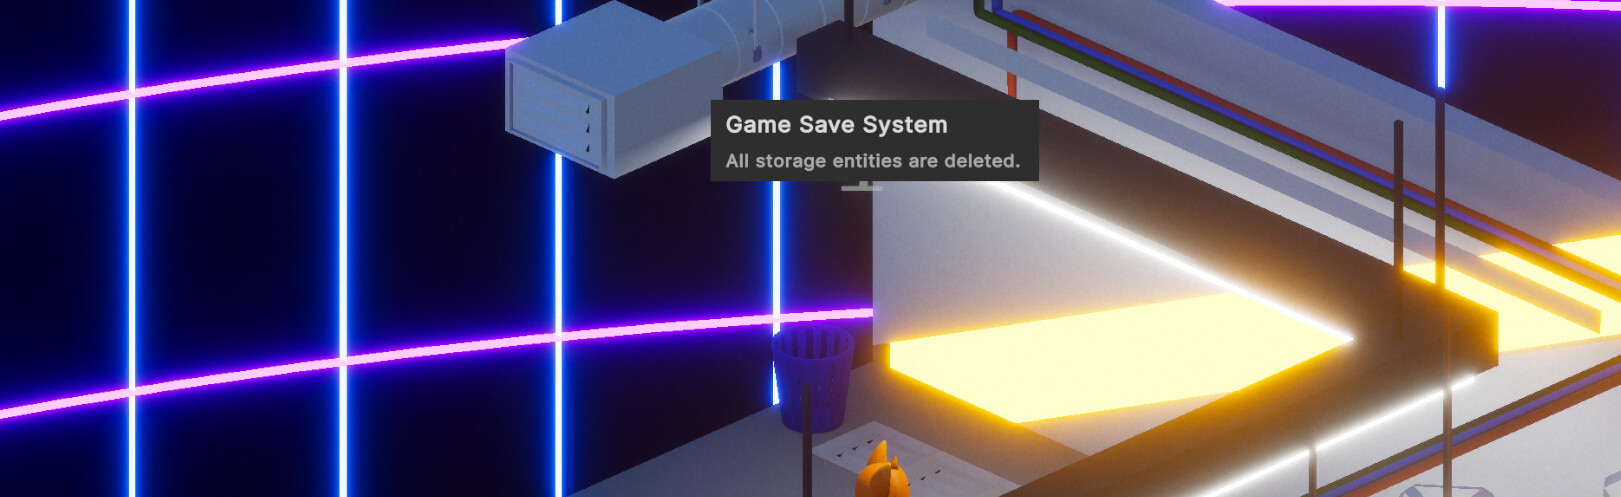
\includegraphics[width=0.8\textwidth]{images/Notificação 1.jpg}
    \caption{Notificação - Destruir todos os servidores.}
    \label{Notificacao_1}
\end{figure}

\begin{figure}[H]
    \centering
    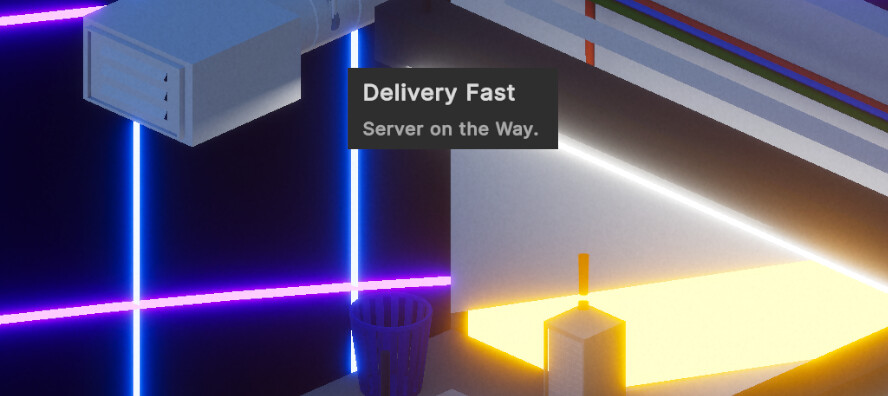
\includegraphics[width=0.8\textwidth]{images/Notificações 2.jpg}
    \caption{Notificação - Compra de um novo servidor.}
    \label{Notificacao_2}
\end{figure}

As Figuras \ref{Notificacao_1} e \ref{Notificacao_2} exemplificação como as notificações são
executadas durante o ciclo de \textit{gameplay}.

\subsection{Referências para a criação de elementos de Jogo e 3D}

No processo de criação de elementos de jogo, sobretudo elementos 3D de cenário, houve o cuidado de utilizar referências reais, como por exemplo, fotos de data centers reais, para a construção dos elementos do jogo, no sentido de criar uma experiência mais imersiva para o jogador, além de possibilitar a criação de conexões entre o jogo e o mundo real, o que se torna benéfico para a construção de uma experiência mais lúdica além de facilitar conexões entre o jogo e jogadores que tenham interesse na temática do jogo, ou que tenham experiência prévia.

No entanto, houve uma adaptação dos mesmos, e uma adição de elementos de fantasia, para criar um ambiente mais divertido e envolvente para o jogador, além de proporcionar uma experiência mais dinâmica e variada.

Neste sentido, houve uma pesquisa prévia sobre a estrutura física de um data center, o que resultou num conjunto de elementos de cenário, que são bastante específicos, destes ambientes. Tais como:
\begin{itemize}
    \item Pavimento técnico;
    \item Racks de servidores;
    \item Cabos de rede;
    \item Sistemas de refrigeração;
    \item Geradores de energia;
    \item Equipamentos de rede;
\end{itemize}

\begin{figure}[H]
    \centering
    \begin{minipage}{0.48\textwidth}
        \centering
        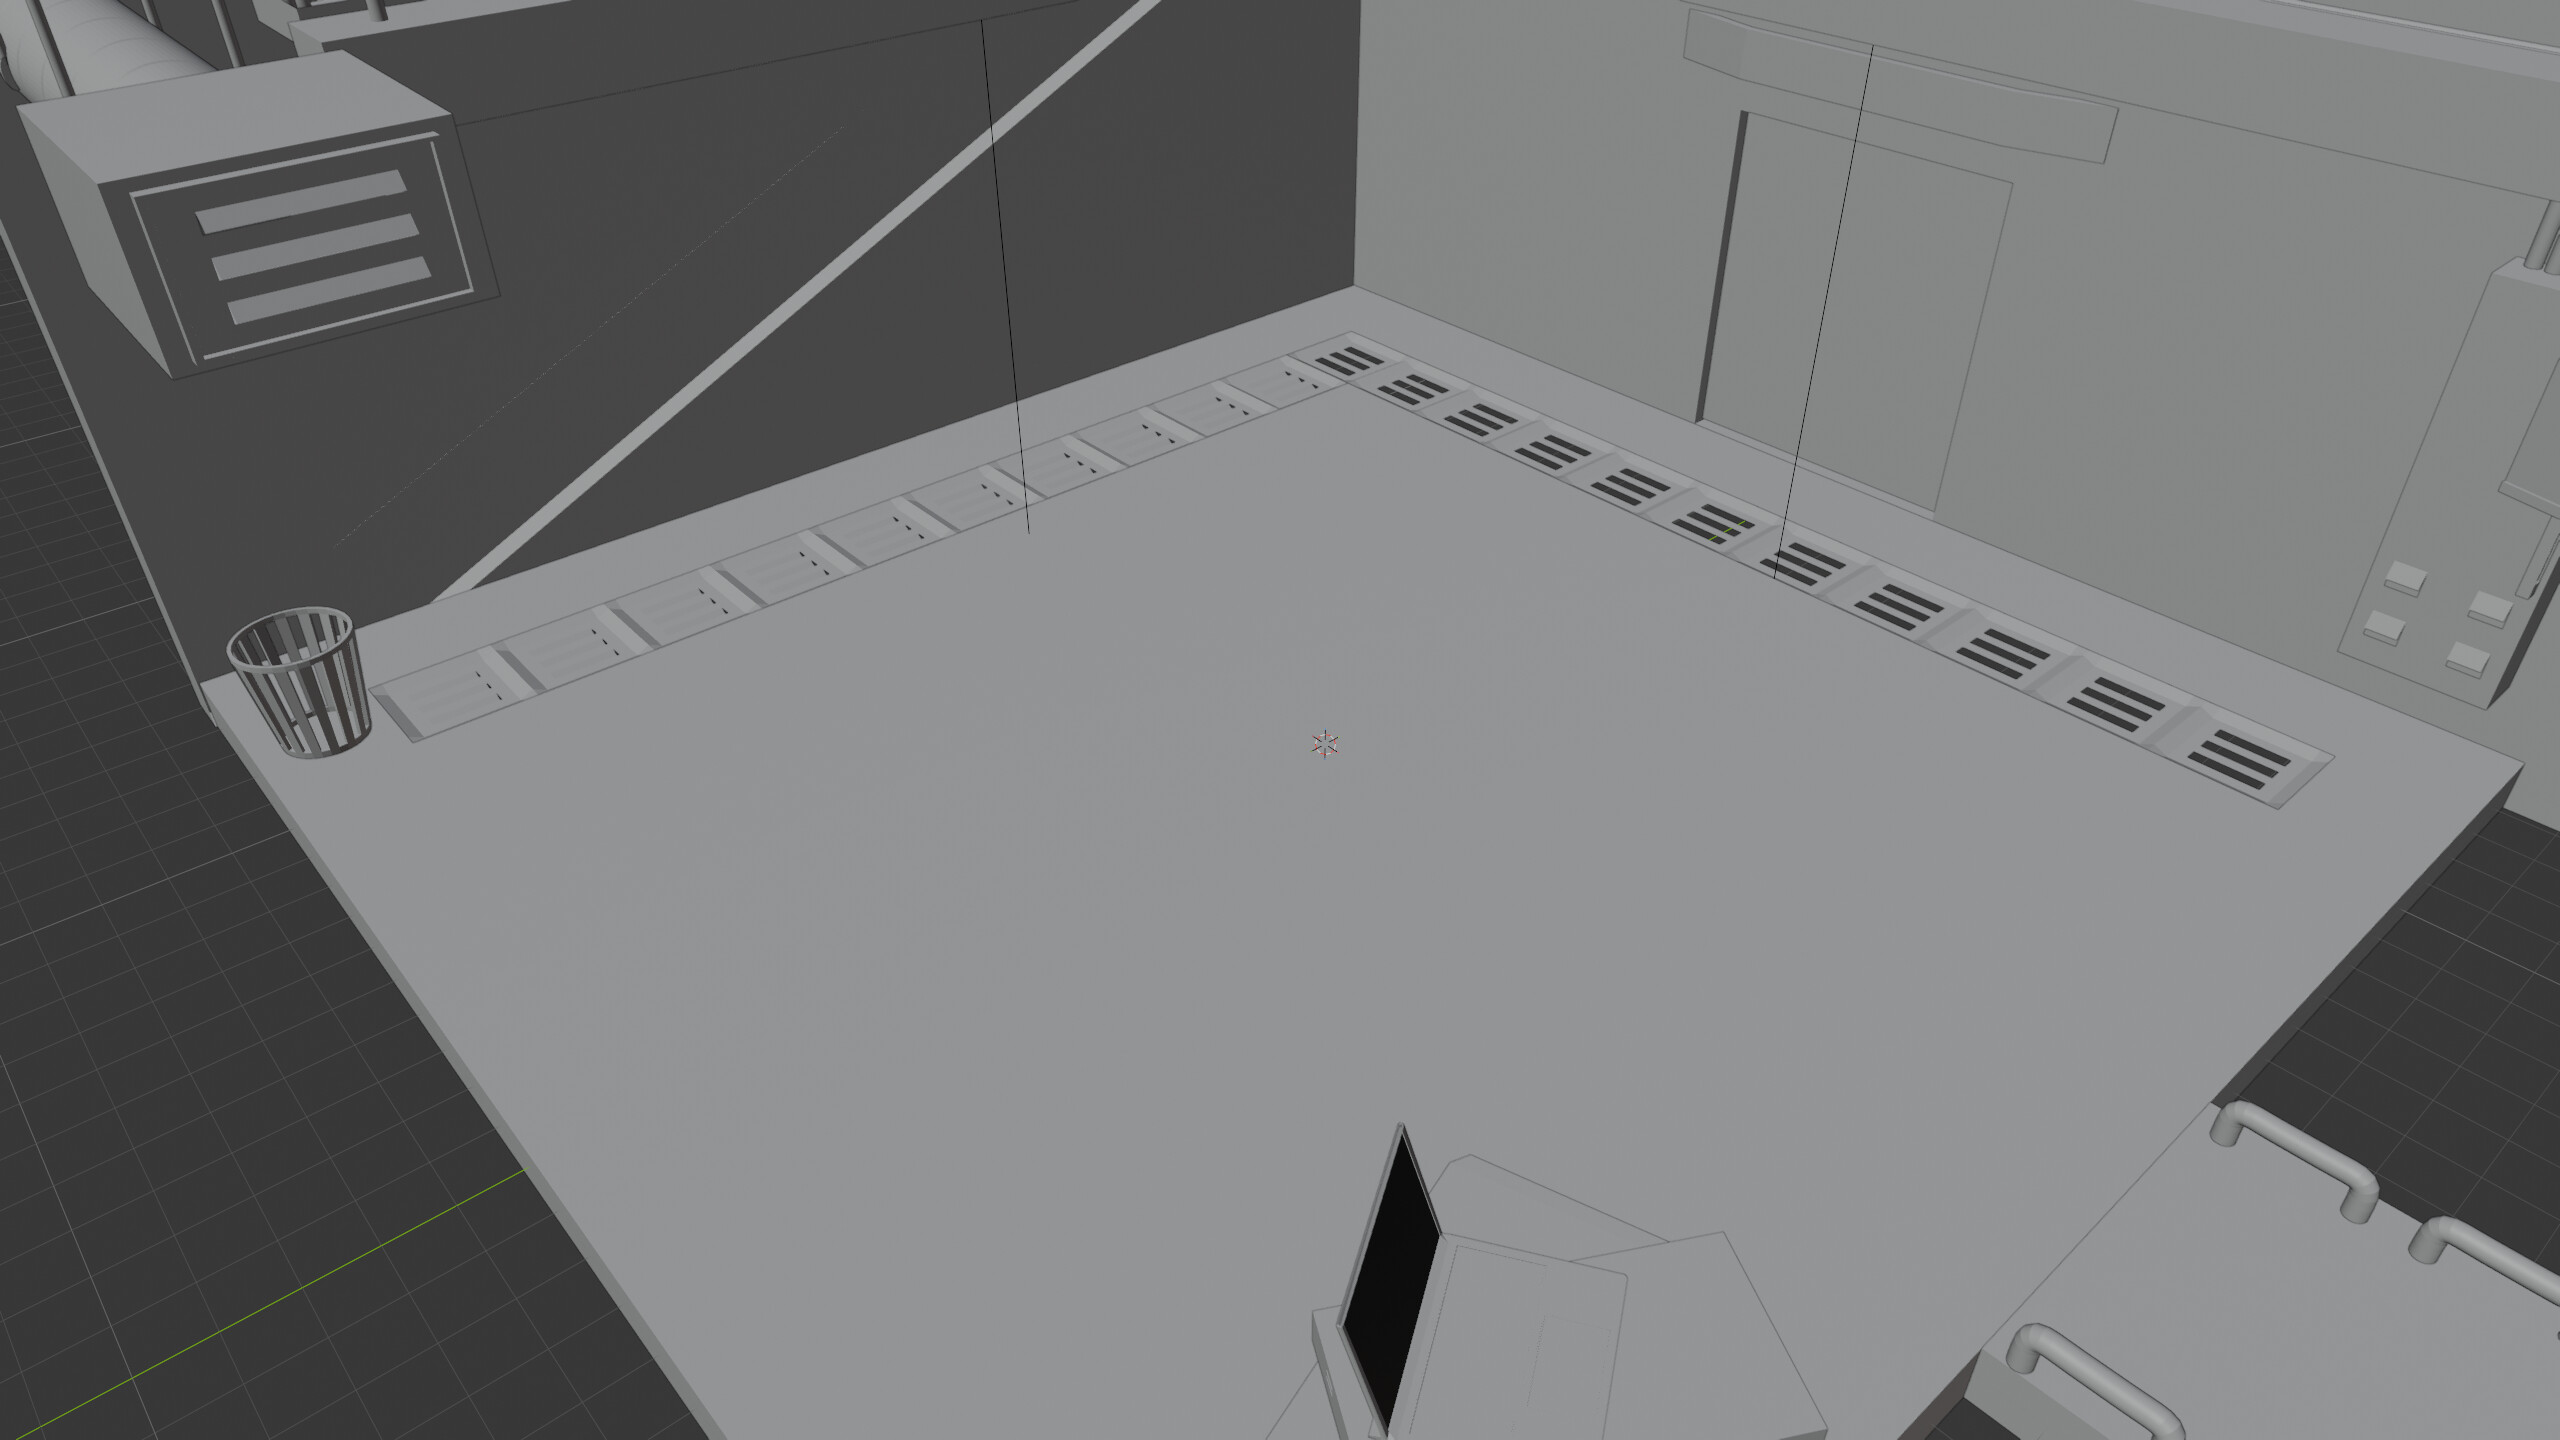
\includegraphics[width=\textwidth]{images/Floor_ViewPort.jpg}
        \caption{Vista de \textit{Viewport} do piso do cenário do jogo.}
        \label{FloorCenarioViewPort}
    \end{minipage}
    \hfill
    \begin{minipage}{0.48\textwidth}
        \centering
        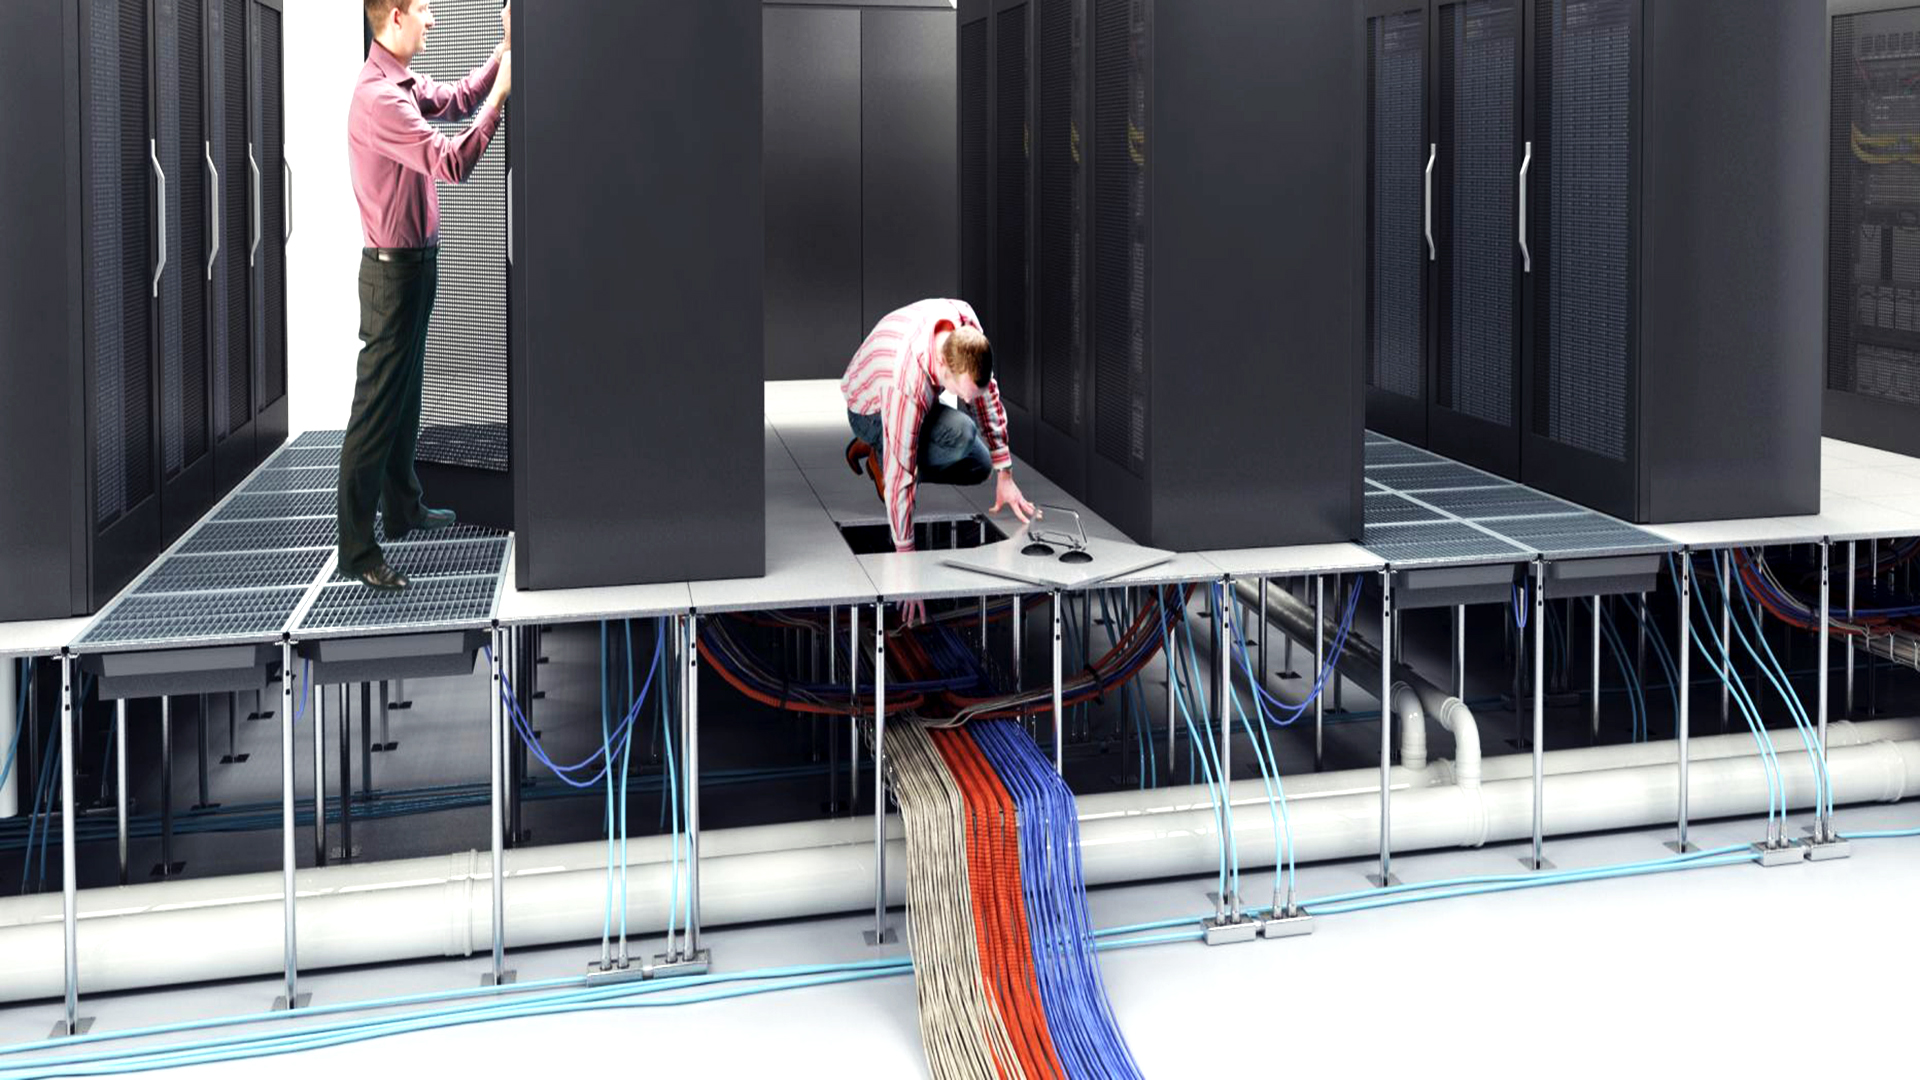
\includegraphics[width=\textwidth]{images/Pavimento Tecnico.jpg}
        \caption{Ilustração do pavimento técnico.}
        \label{PavimentoTecnico}
    \end{minipage}
\end{figure}

Analisando o cenário da Figura \ref{FloorCenarioViewPort} é possível observar a presença de umas caixas no chão, que apresenta algumas perfurações, estas caixas têm como finalidade representar o pavimento técnico ou pavimento elevado, representado na Figura \ref{PavimentoTecnico}, que é um elemento comum em data centers, e tem a função de permitir a passagem de cabos e sistemas de refrigeração, além de facilitar o acesso aos equipamentos instalados no chão do data center.
A representação no jogo é uma adaptação do pavimento técnico real, onde as caixas foram simplificadas, e a fiação de cabos fui desconsiderada. A sua localização no cenário, também serve de marcação para o jogador, uma vez que sempre que existe a compra de um novo servidor, o mesmo é colocado atrás de uma dessas caixas.

\begin{figure}[H]
    \centering
    \begin{minipage}{0.48\textwidth}
        \centering
        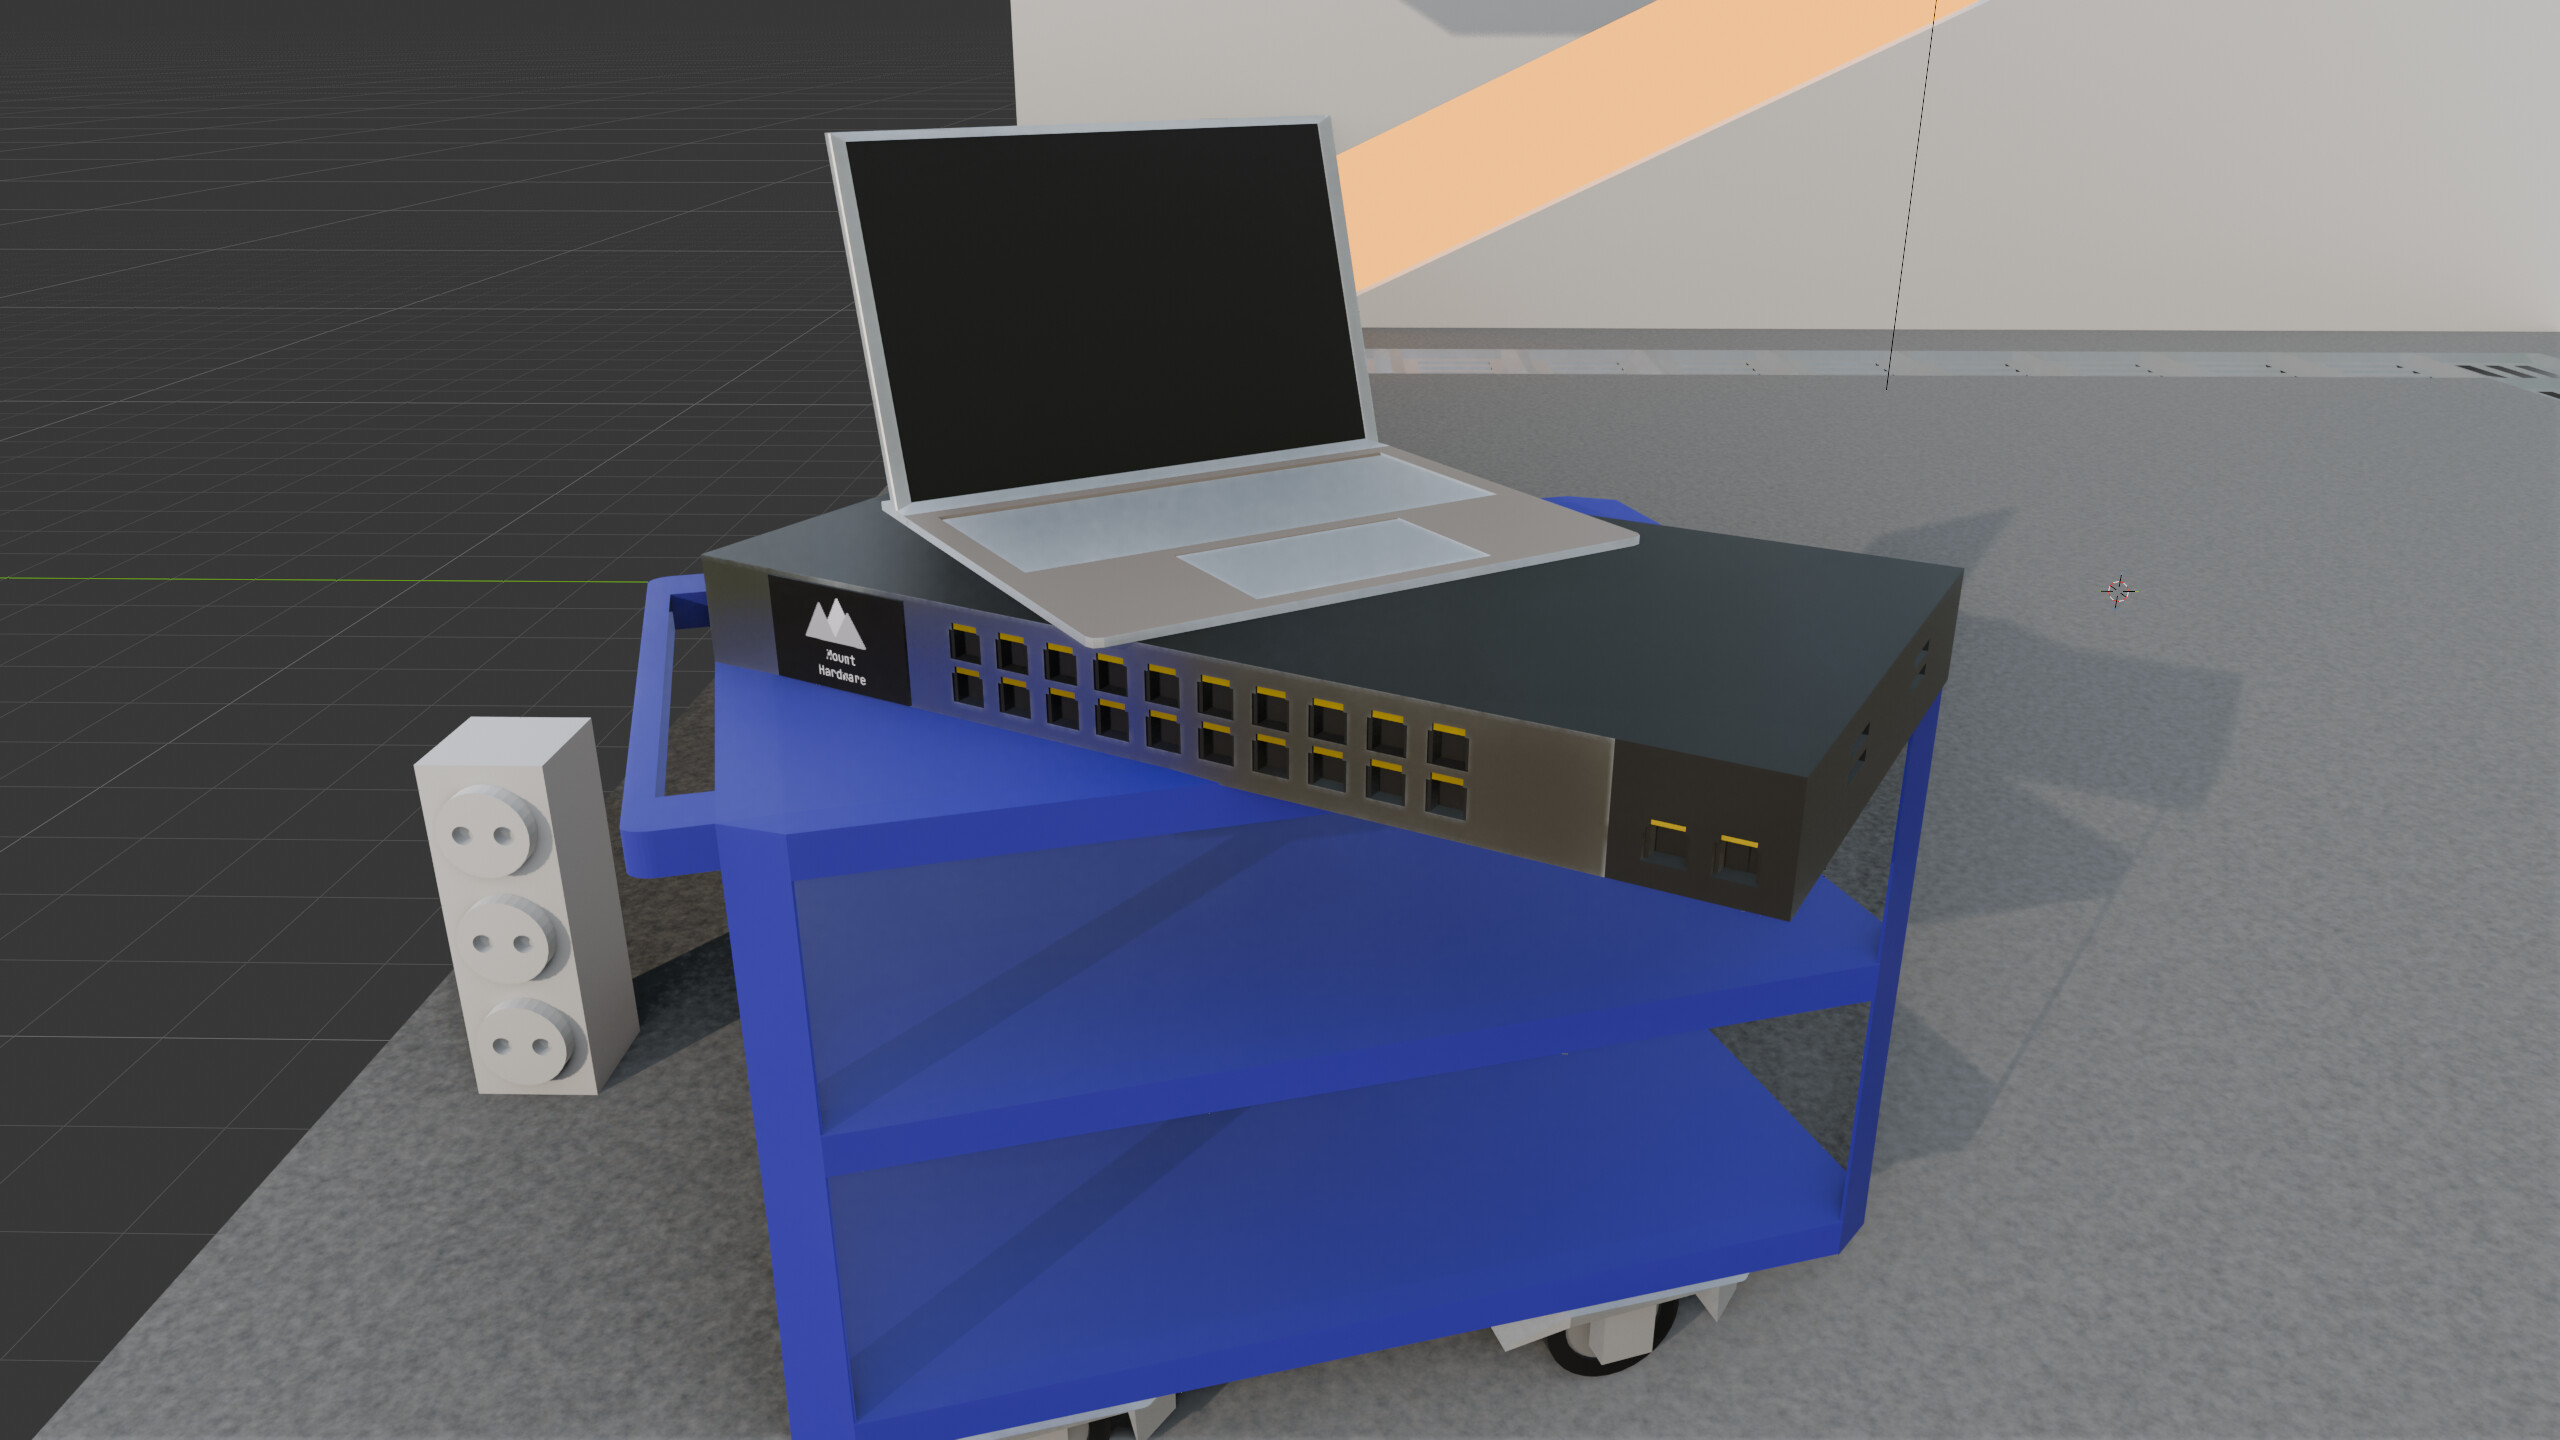
\includegraphics[width=\textwidth]{images/SwitchViewPort.jpg}
        \caption{Vista de \textit{Viewport} do switch de rede.}
        \label{SwitchCenarioViewPort}
    \end{minipage}
    \hfill
    \begin{minipage}{0.48\textwidth}
        \centering
        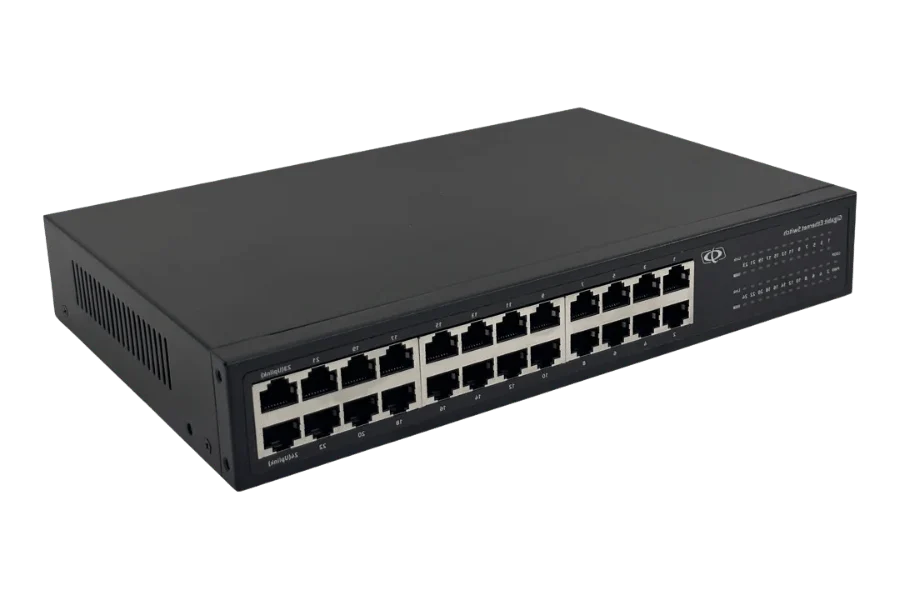
\includegraphics[width=\textwidth]{images/Switch.png}
        \caption{Ilustração do switch de rede.}
        \label{Switch}
    \end{minipage}
\end{figure}

Além da estrutura do próprio cenário, os elementos de decoração presentes nele, são igualmente relevantes para a caracterização do espaço. Assim sendo houve o cuidado de criar elementos que remetem para o contexto de data center, tais como o switch representando na Figura \ref{SwitchCenarioViewPort}. O switch é um equipamento de rede utilizado para conectar vários dispositivos em uma mesma rede local. A representação do switch no jogo é uma adaptação de um switch real, mostrado na figura \ref{Switch}.

\begin{figure}[H]
    \centering
    \begin{minipage}{0.48\textwidth}
        \centering
        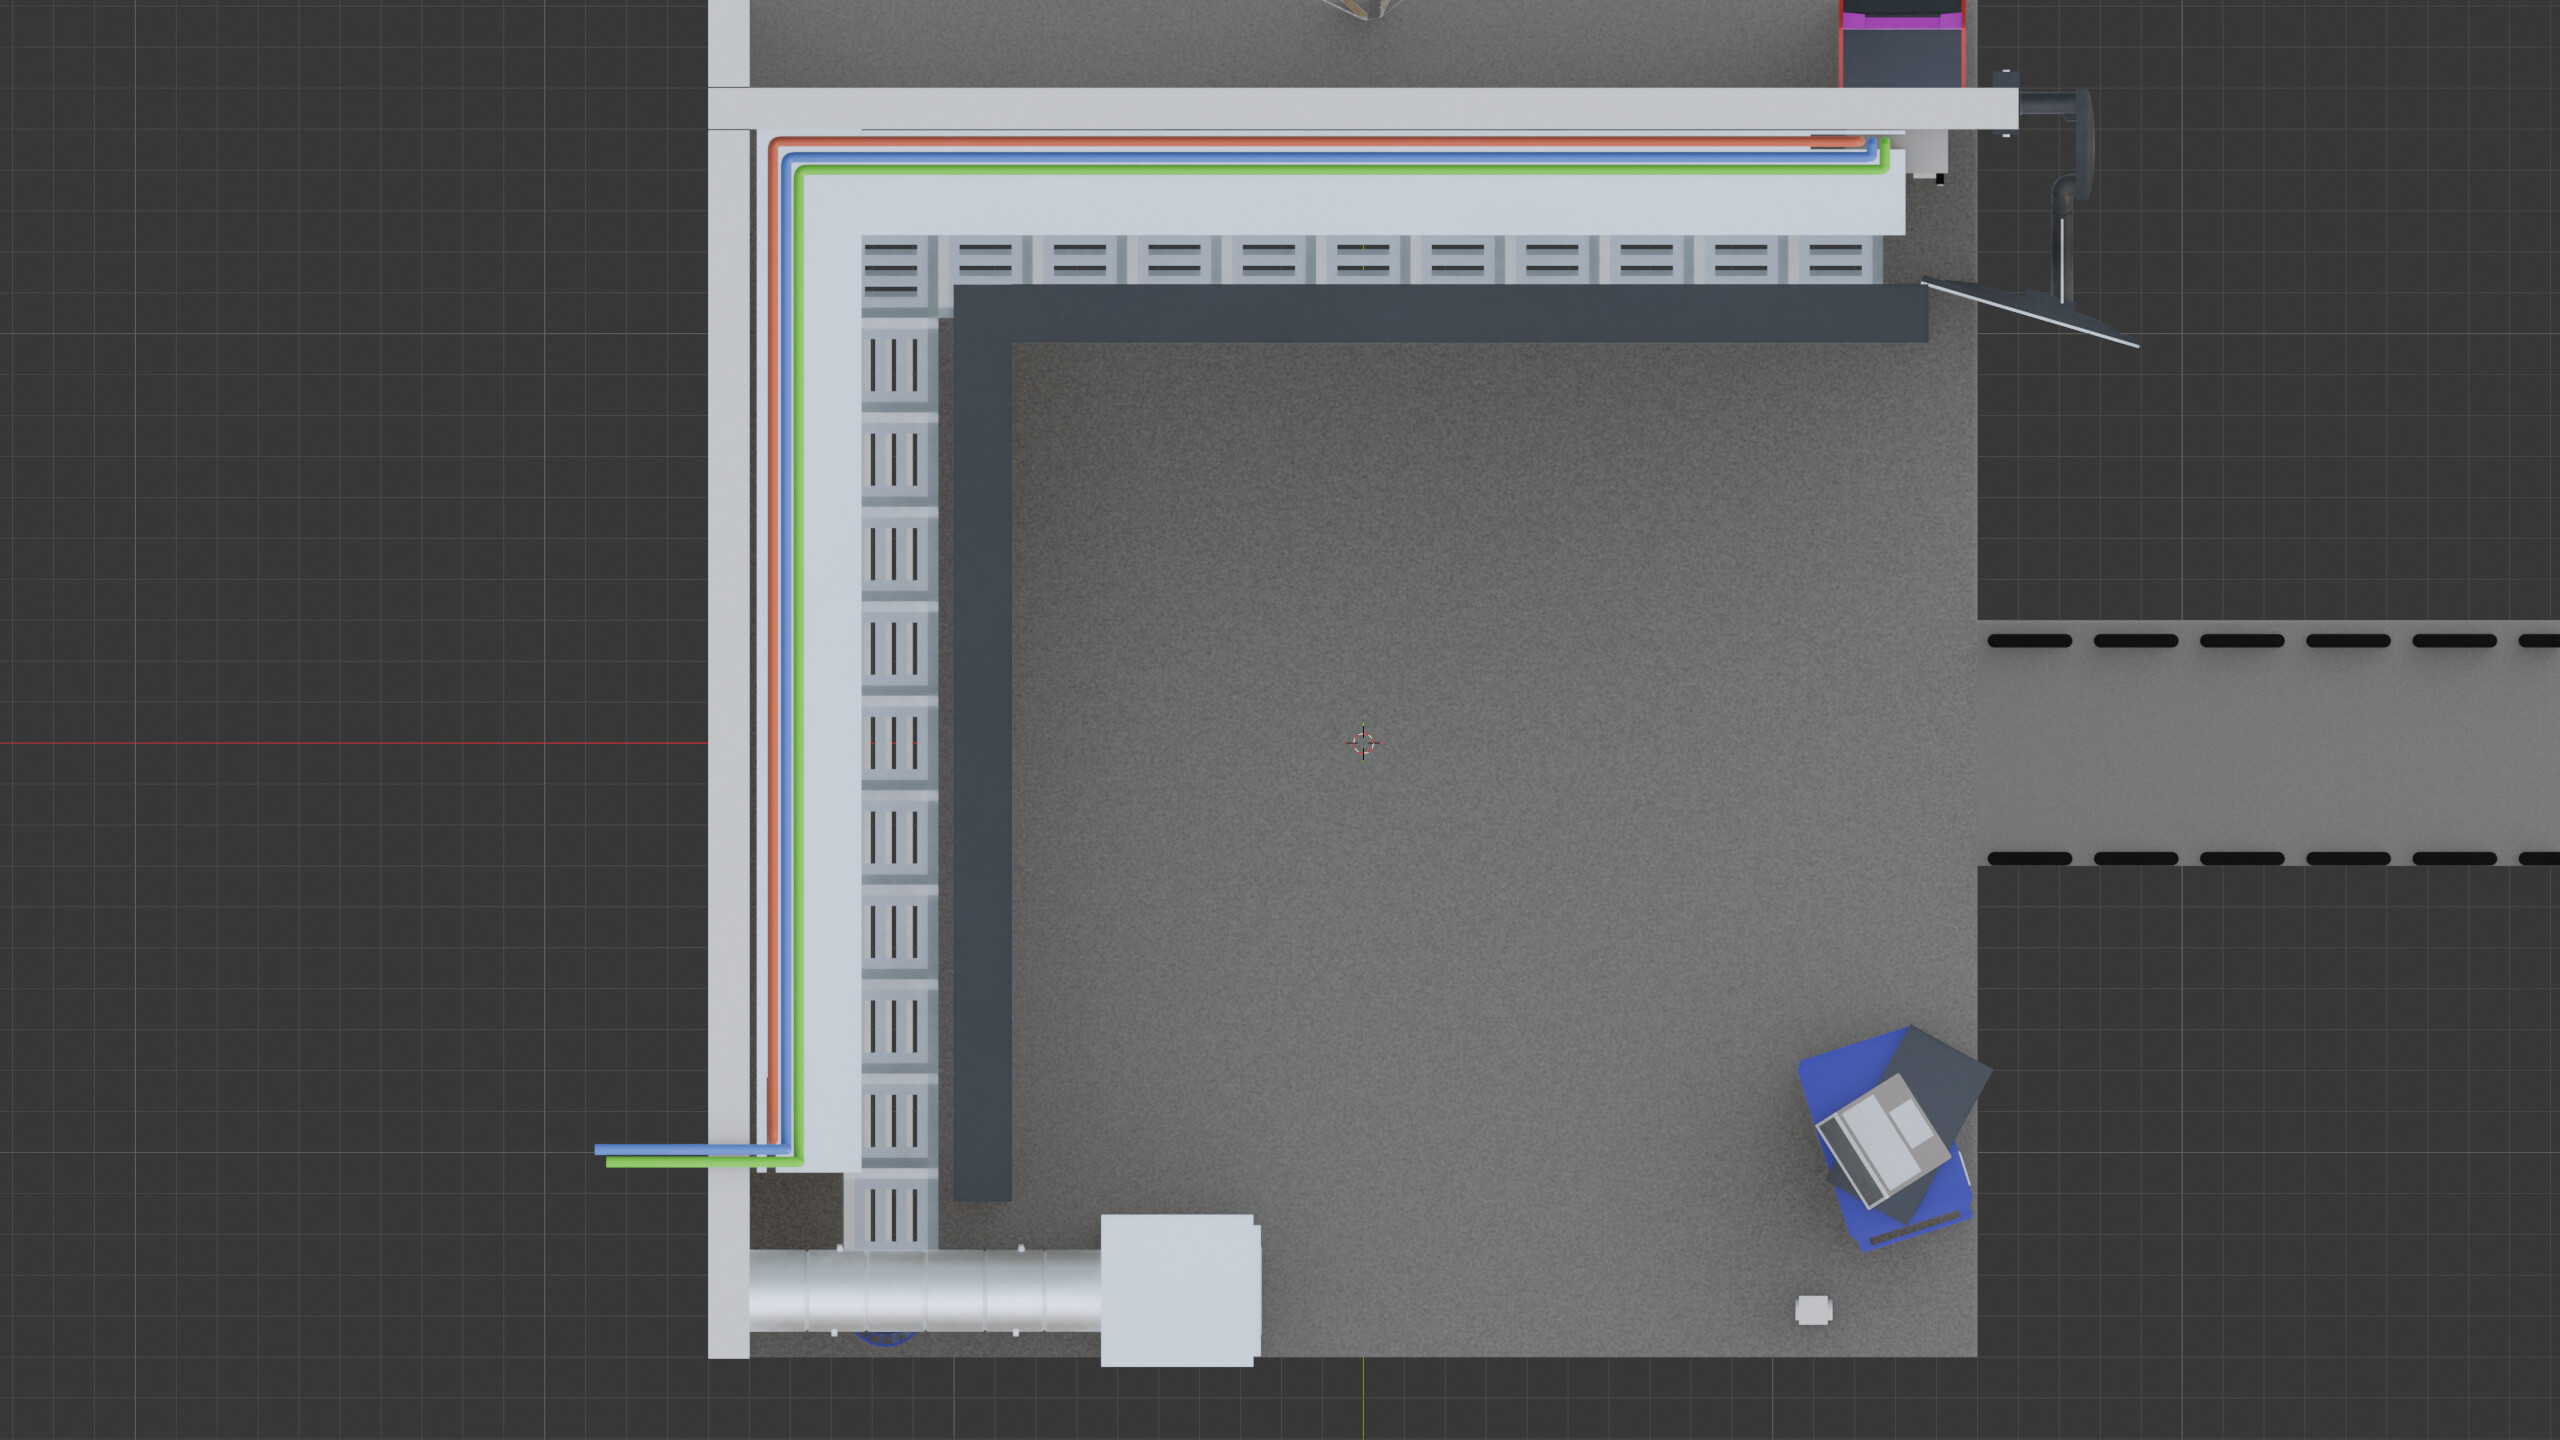
\includegraphics[width=\textwidth]{images/CabesViewPort.jpg}
        \caption{Vista de \textit{Viewport} do caminho de cabos (Vista de cima).}
        \label{CabesCenarioViewPort}
    \end{minipage}
    \hfill
    \begin{minipage}{0.48\textwidth}
        \centering
        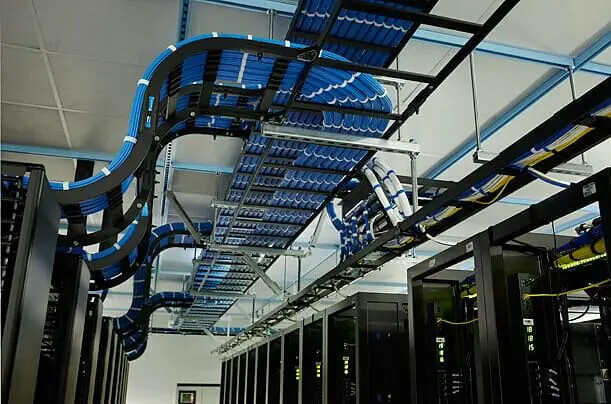
\includegraphics[width=\textwidth]{images/CaminhoCabos.jpg}
        \caption{Ilustração do caminho dos cabos.}
        \label{CaminhoCabos}
    \end{minipage}
\end{figure}

Na parte superior do cenário, existe outro detalhe de decoração, bastante importante para a caracterização do espaço, que é o caminho de cabos, representado na Figura \ref{CabesCenarioViewPort}. Um caminho de cabos, é na sua essência, uma calha colocada geralmente no teto, que tem a função de organizar, proteger e transportar os cabos de rede, energia e outros pelo espaço do data center.
Na Figura \ref{CaminhoCabos} pode ser vista uma representação realista do mesmo.

Na Figura \ref{CabesCenarioViewPort} é possível observar uma representação de um sistema de ventilação e refrigeração, que é um elemento essencial em data centers, uma vez que tem a função de manter a temperatura e a umidade do ambiente controladas, garantindo o bom funcionamento dos equipamentos. A representação do sistema de ventilação e refrigeração no jogo é uma adaptação de um sistema real, onde os detalhes foram simplificados para se adequar ao estilo visual do jogo.

\begin{figure}[H]
    \centering
    \begin{minipage}{0.48\textwidth}
        \centering
        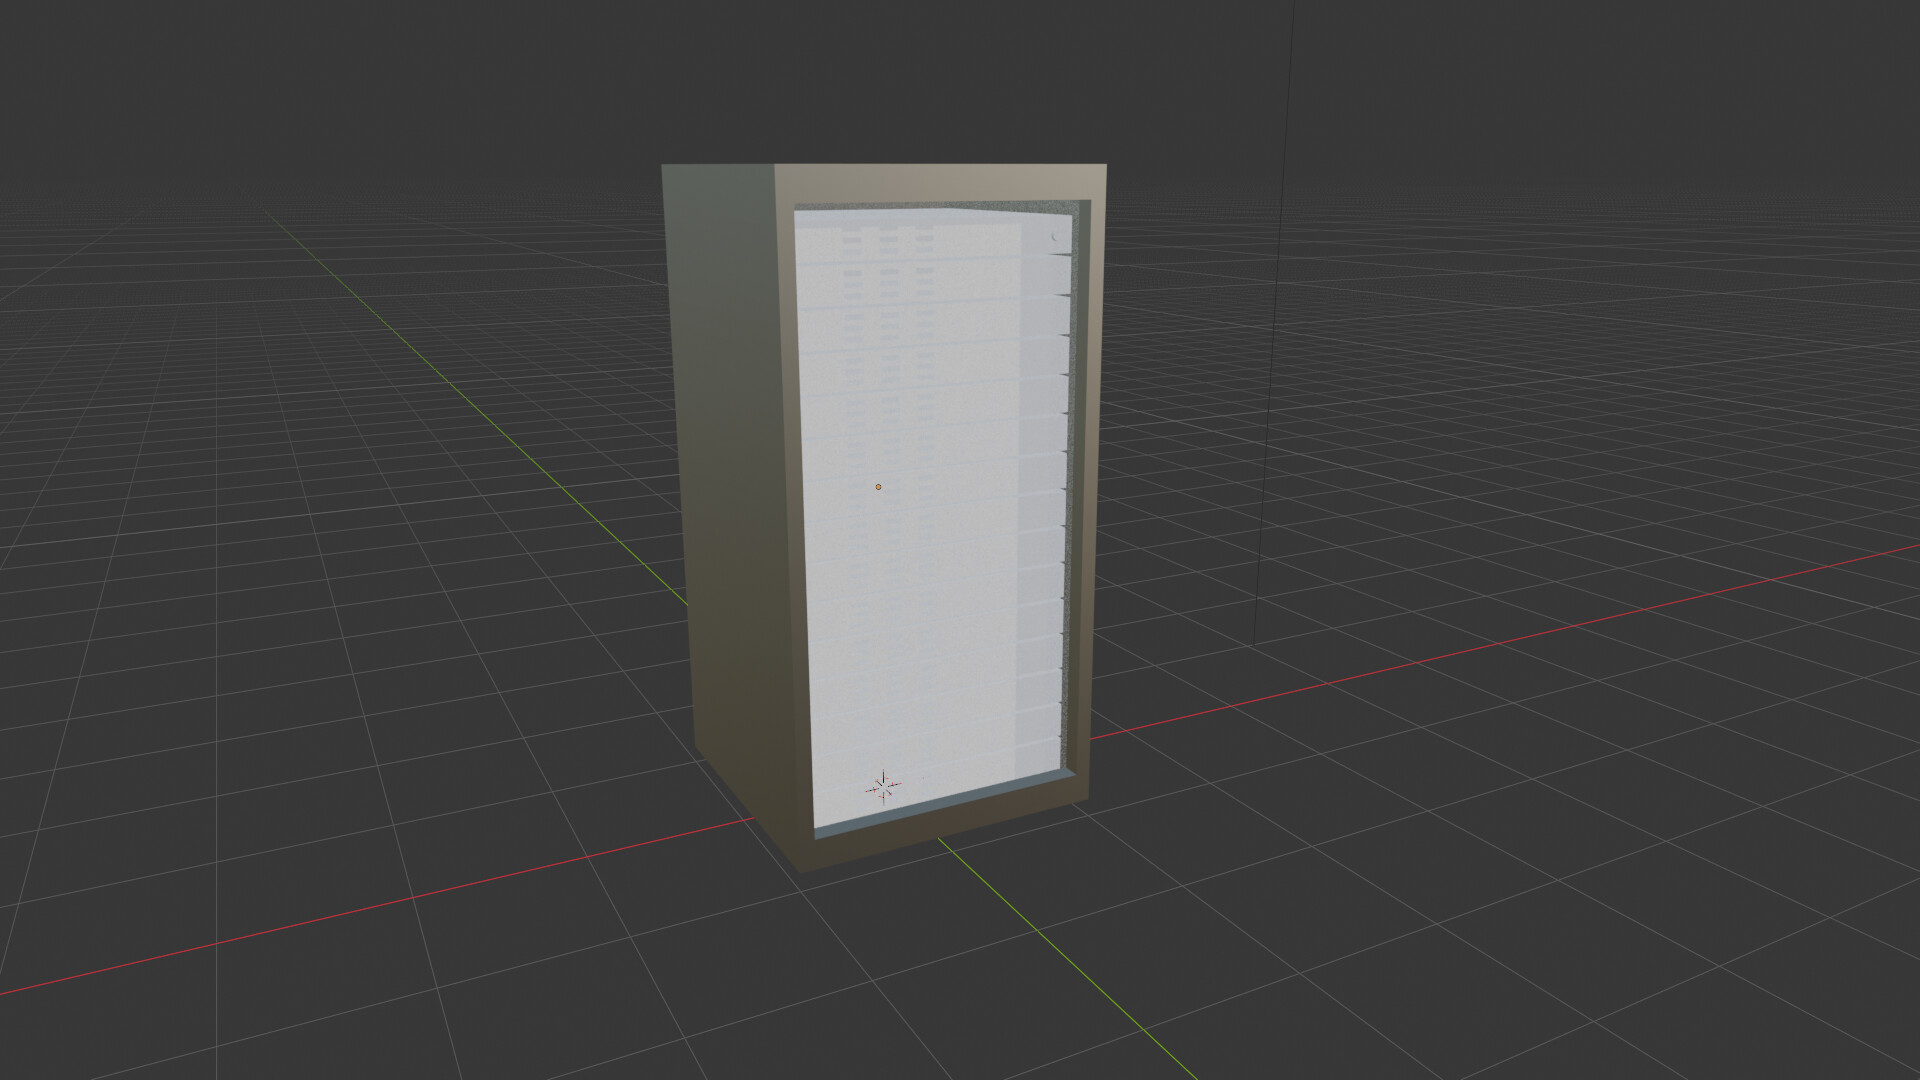
\includegraphics[width=\textwidth]{images/ServidorViewPort.jpg}
        \caption{Vista de \textit{Viewport} do servidor.}
        \label{ServidorViewPort}
    \end{minipage}
    \hfill
    \begin{minipage}{0.48\textwidth}
        \centering
        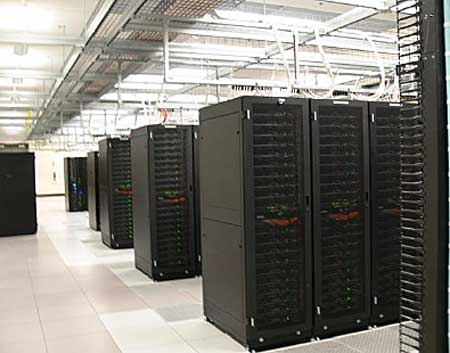
\includegraphics[width=\textwidth]{images/Servidor_Amazon.jpg}
        \caption{Representação do servidor da Amazon.}
        \label{ServidorAmazon}
    \end{minipage}
\end{figure}

A representação de servidores no jogo, assim como se pode ver na Figura \ref{ServidorViewPort}, é uma adaptação de \textit{racks} de servidores reais, conforme é mostrado na Figura \ref{ServidorAmazon}. Os \textit{racks} de servidores são estruturas metálicas que abrigam os equipamentos de um data center, como servidores, switches, roteadores, etc... A representação de servidores no jogo, foi simplificada, no sentido de homogeneizar a aparência de todos os equipamentos e função os limitando apenas servidores, no sentido de computadores.

\begin{figure}[H]
    \centering
    \begin{minipage}{0.48\textwidth}
        \centering
        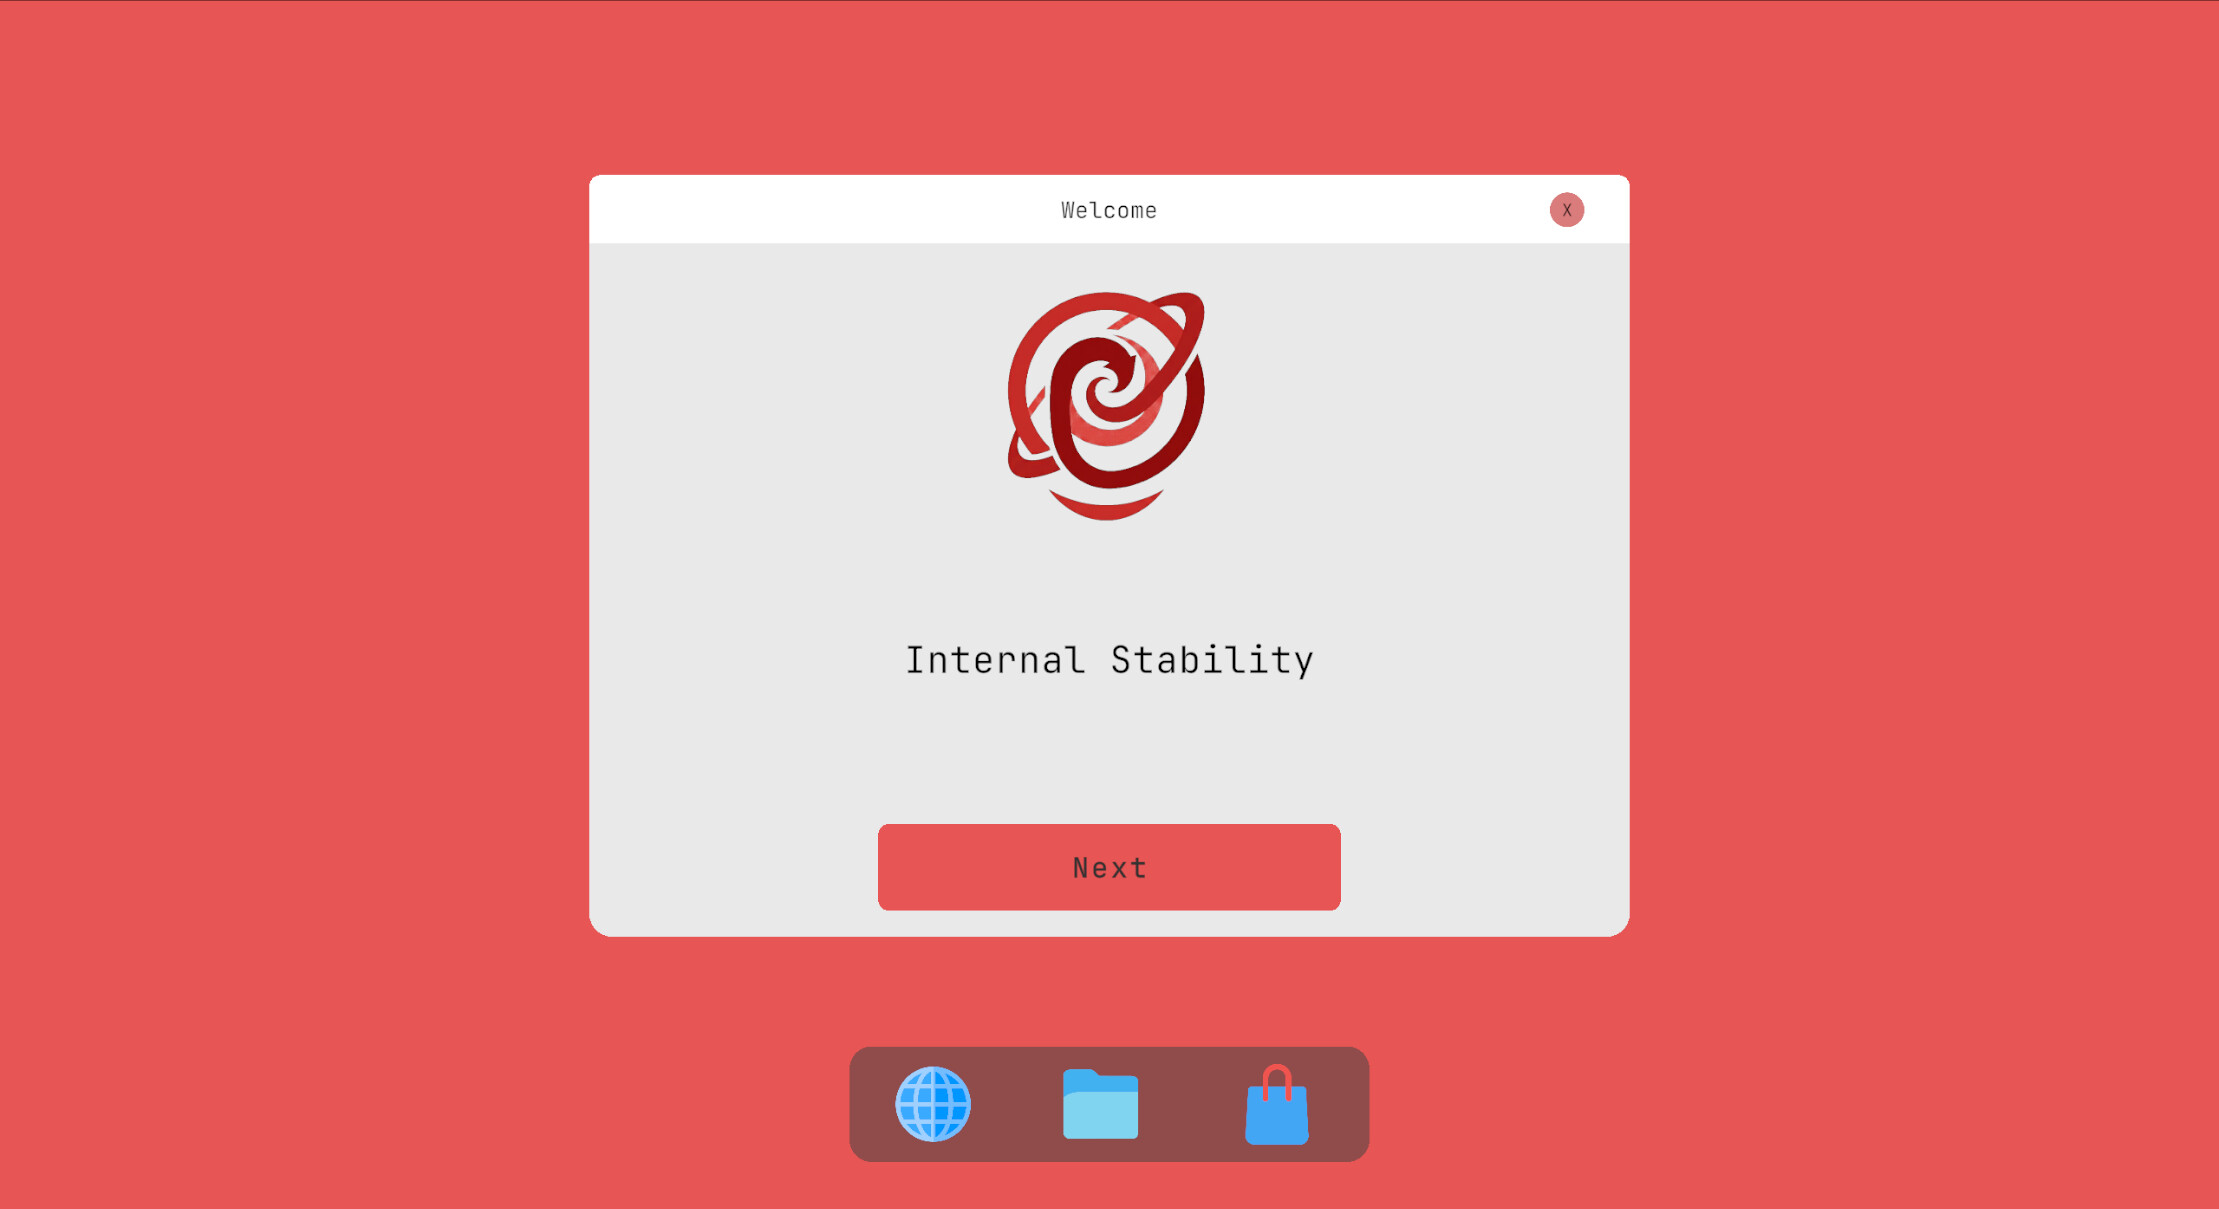
\includegraphics[width=\textwidth]{images/GnomeGame.jpg}
        \caption{\textit{UI} da instalação e configuração de um sistema operativo.}
        \label{GameGnomeUI}
    \end{minipage}
    \hfill
    \begin{minipage}{0.48\textwidth}
        \centering
        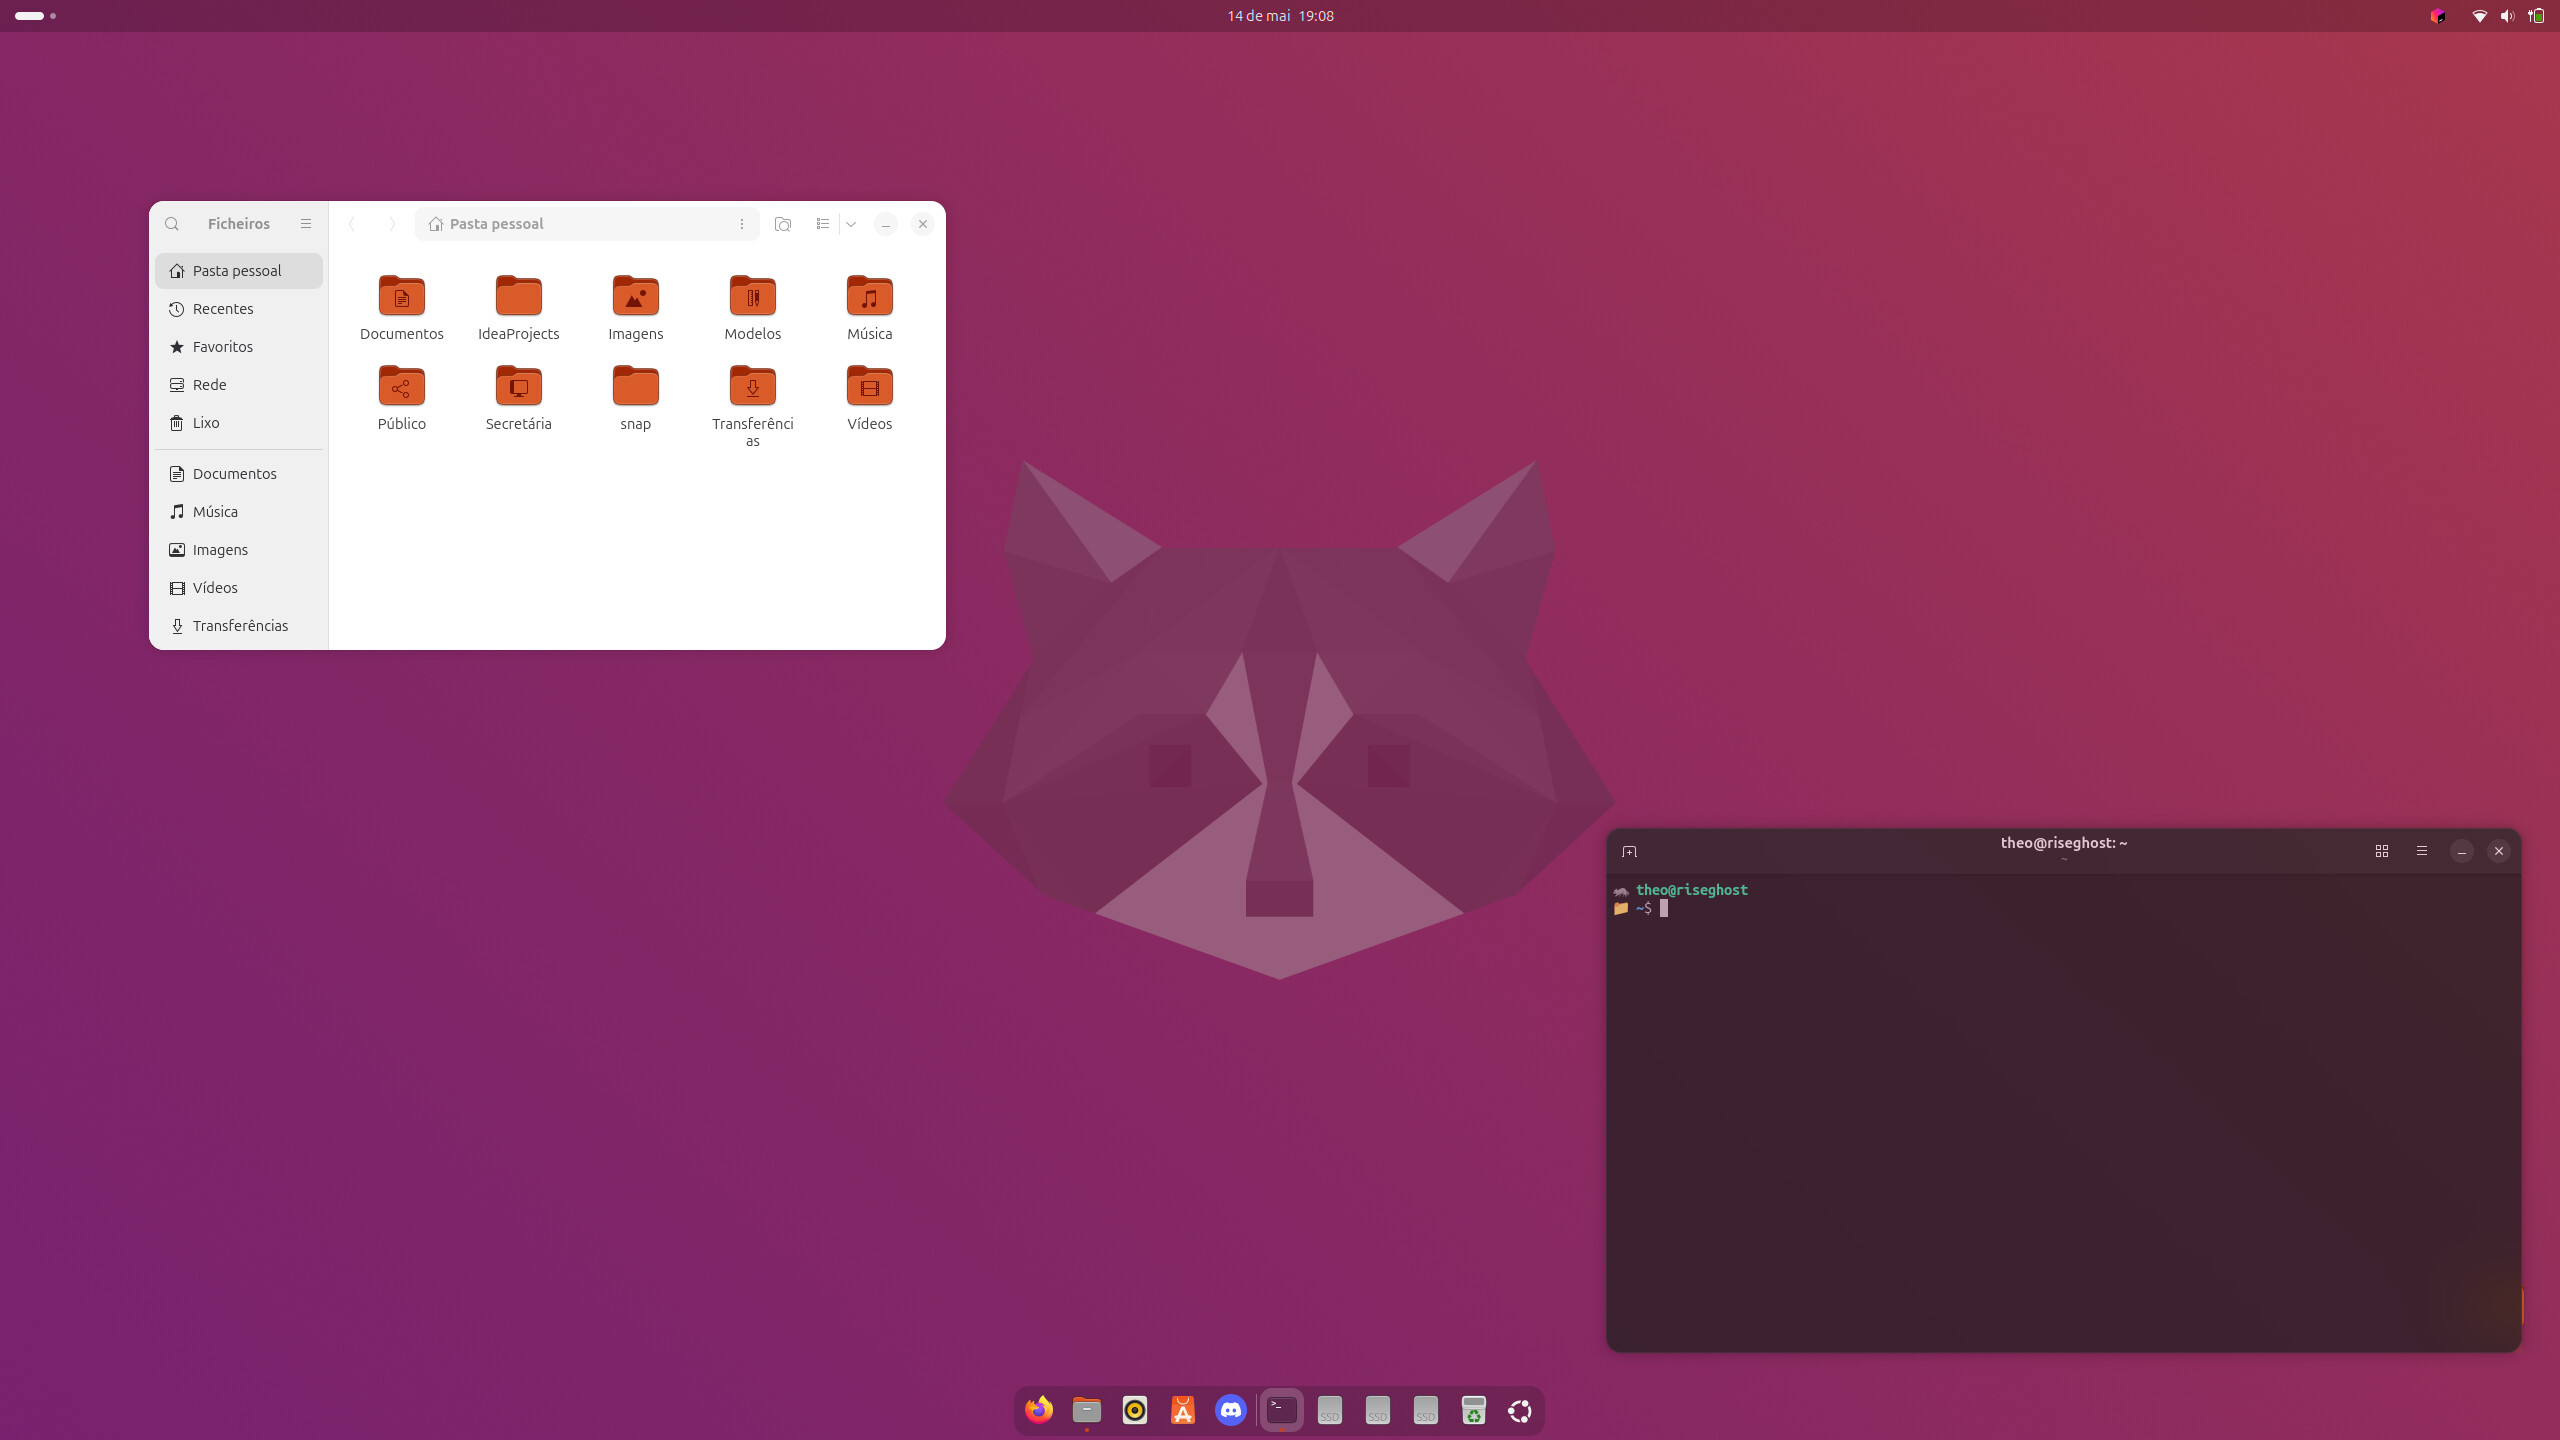
\includegraphics[width=\textwidth]{images/Imagem colada.jpg}
        \caption{Ambiente gráfico Gnome.}
        \label{GnomeUI}
    \end{minipage}
\end{figure}

Por fim, além de elementos gráficos de cenário, elementos de \textit{UI}, tais como a interface de configuração de um sistema operativo, foram igualmente inspirados em referência reais.
Na Figura \ref{GnomeUI} é mostrado a interface gráfica Gnome, que é um ambiente gráfico vastamente utilizado em sistemas operativos Linux, embora a sua utilização em data centers não seja tão comum, ainda assim, é bastante dissolvida no ambiente de tecnologia.
Devia a ser uma interface gráfica mais amigável e intuitiva, servi como inspiração para a construção da interface vista na Figura \ref{GameGnomeUI}.

\section{Desenvolvimento do conceito de jogo}

Este projeto consiste na construção de um vídeo jogo, onde o jogador é responsável
por fazer a gestão de um pequeno data center, onde o objetivo é ganhar dinheiro.

No entanto, durante todo o percurso de \textit{gameplay}, o jogador terá várias etapas a cumprir,
como, comprar equipamento, configurar o equipamento, resolução de pequenos
puzzles disponibilizados sobre a forma de \textit{mini games}, gestão de recursos económicos e 
combate contra ameaças, como, por exemplo, vírus e ataques de \textit{hackers}.

Nas subseções seguintes, será desenvolvido de forma mais detalhada cada um dos pontos
principais do conceito do jogo.

\subsection{Compra e configuração de equipamento}

Durante a compra de equipamentos para o data center, o jogador tem a sua disposição uma interface completa de
configuração, onde é possivel escolher componentes como:
\begin{itemize}
    \item Processadores;
    \item RAM;
    \item Discos de vários tipos;
    \item Placas de rede;
    \item Sistema Operativo;
    \item Sistemas de refrigeração (Está presente de forma simplificada).
\end{itemize}

\begin{figure}[H]
  \centering
  % --- Primeira Figura (Métricas) ---
  \begin{minipage}[b]{0.48\textwidth}
    \centering
    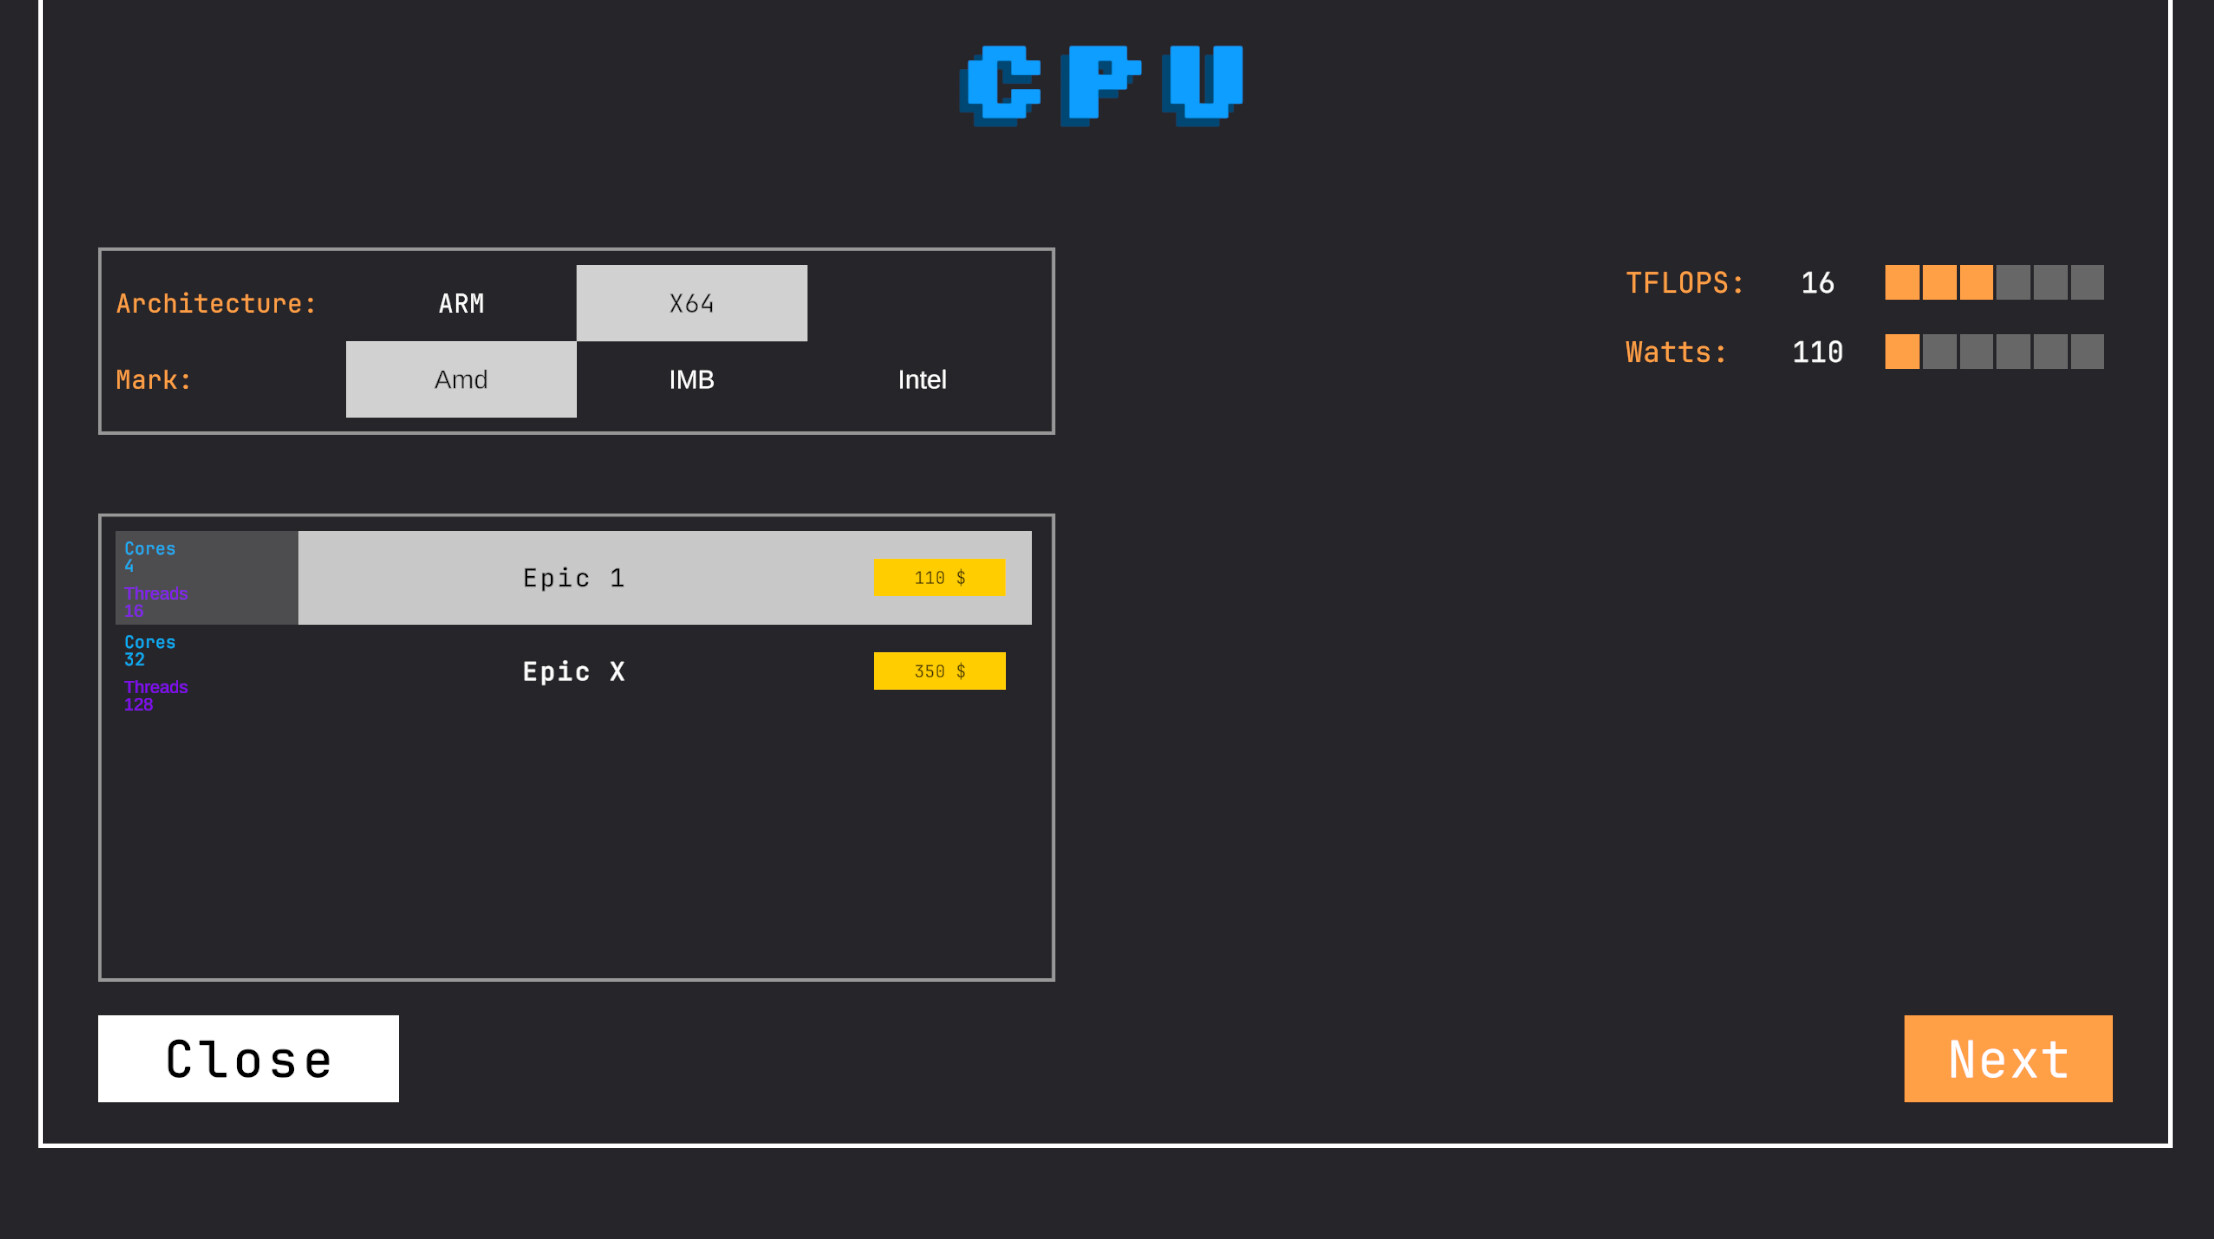
\includegraphics[width=\textwidth]{images/Projeto CPU.jpg}
    \caption[Captura de tela do jogo - Configuração de CPU.]{Captura de tela do jogo - Configuração de CPU.}
    \label{Projeto_config_cpu1}
  \end{minipage}
  \hfill % Espaçamento entre as minipages
  % --- Segunda Figura (Servidores) ---
  \begin{minipage}[b]{0.48\textwidth}
    \centering
    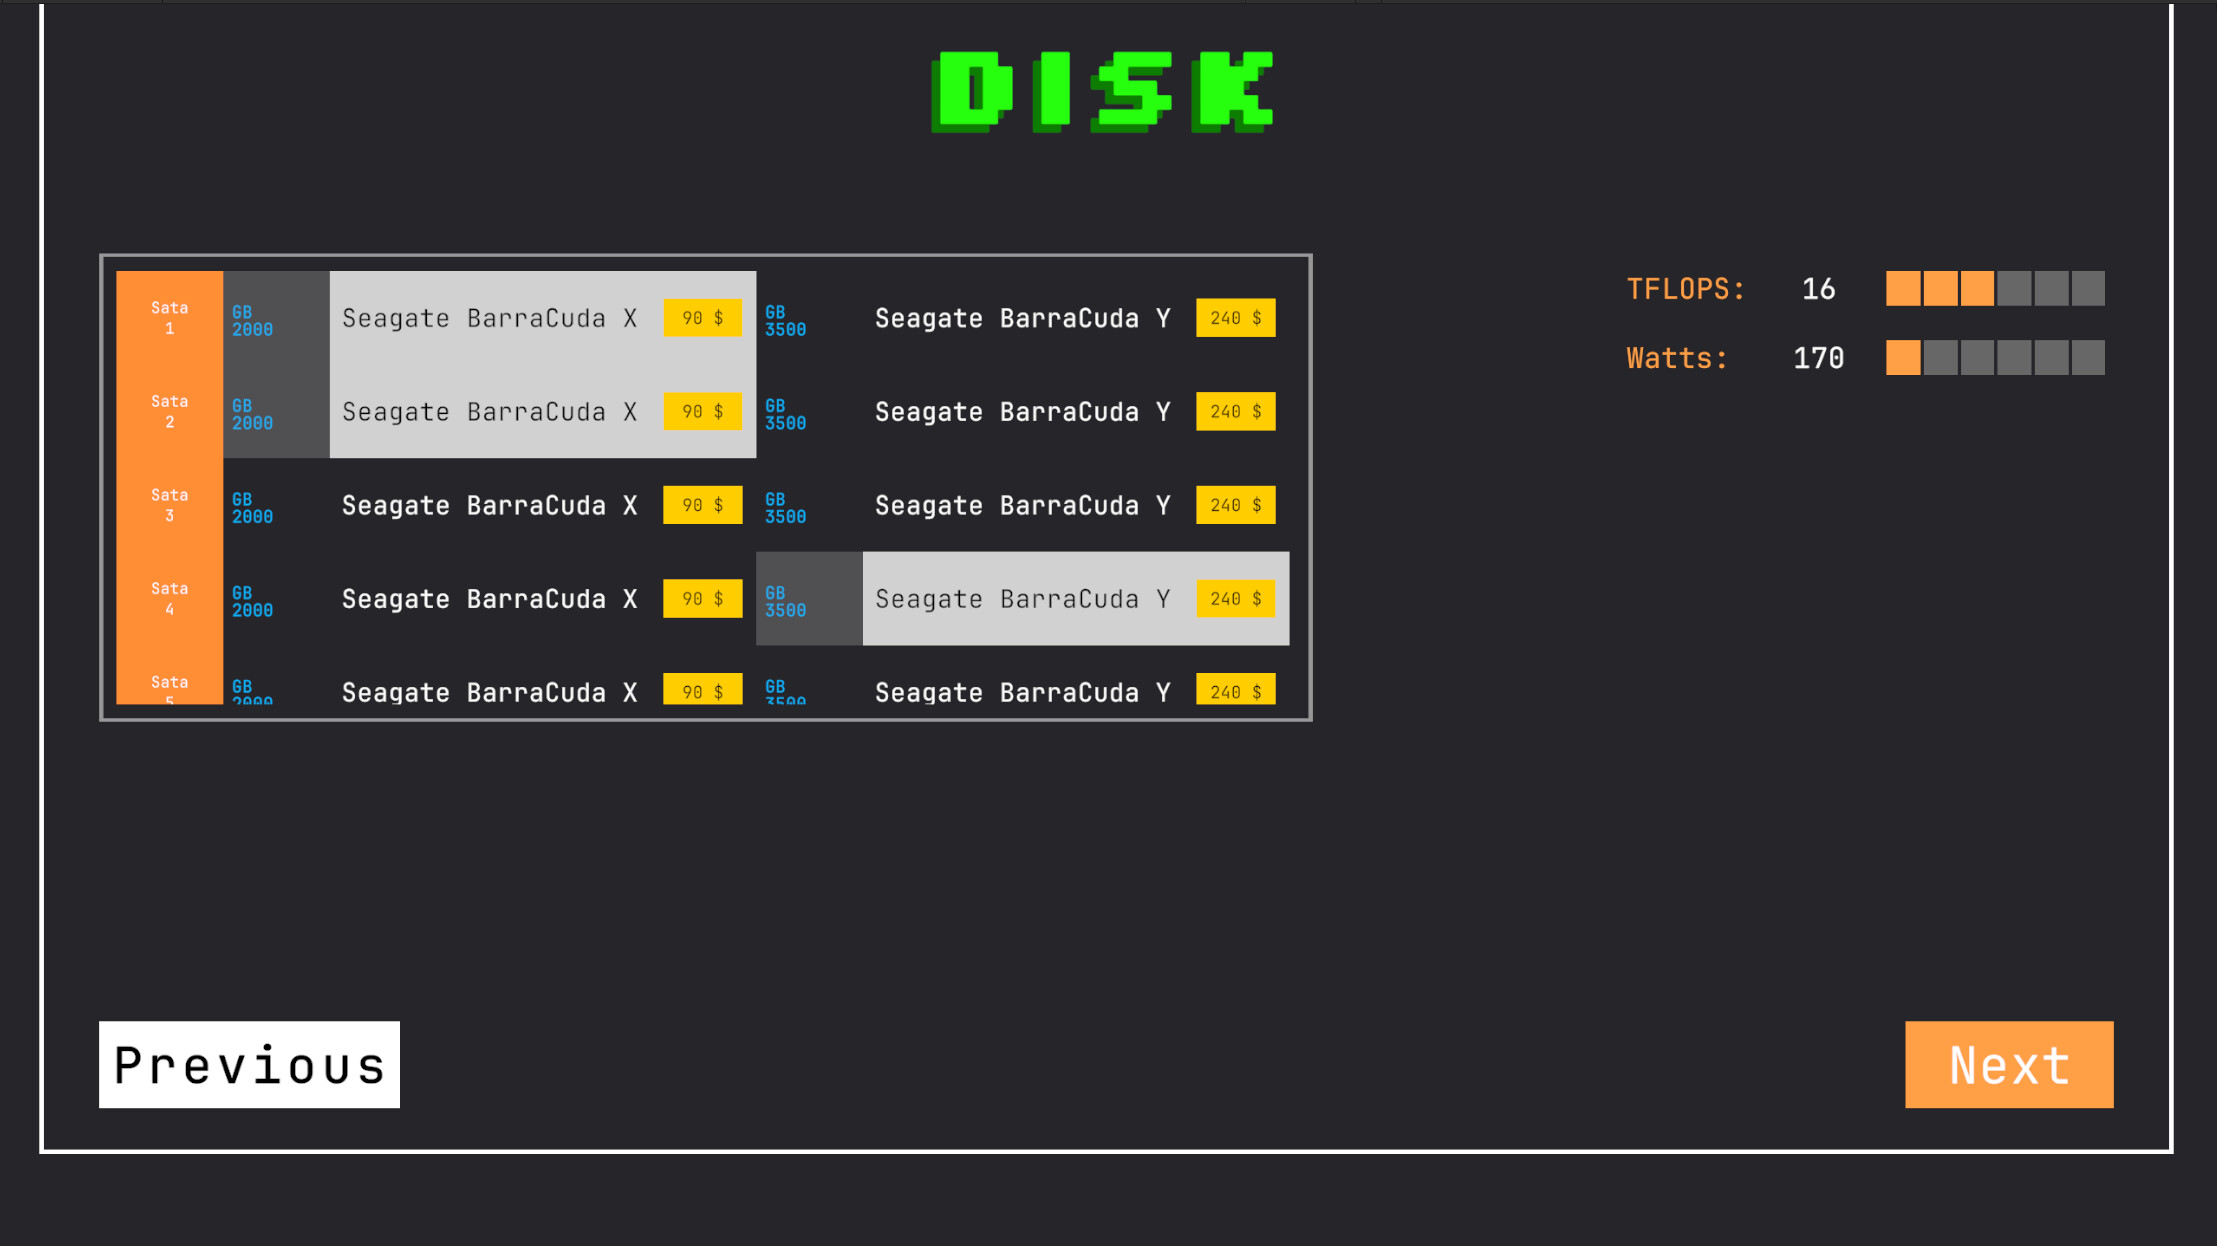
\includegraphics[width=\textwidth]{images/Projeto Disk.jpg}
    \caption[Captura de tela do jogo - Configuração de discos.]{Captura de tela do jogo - Configuração de discos.}
    \label{Projeto_config_disk1}
  \end{minipage}
\end{figure}

Na Figura \ref{Projeto_config_cpu1} e na Figura \ref{Projeto_config_disk1} 
é possível observar a interface de configuração de CPU e de discos, 
respetivamente, onde o jogador tem a possibilidade de escolher entre vários tipos 
de componentes, cada um com as suas próprias características e preços, 
o que torna a escolha do equipamento uma parte importante da estratégia do jogo.
Além disso, cada componente tem um impacto direto no consumo de energia (\textit{Watts})
assim como no desempenho daquele servidor (\textit{TFLOPS}).
As unidades utilizadas (\textit{Watts} e \textit{TFLOPS}) são unidades reais,
e o uso server para reforma a imersão do jogador, além de tornar o jogo mais
realista, e permitir a adição de conteúdo educativo de forma lúdica. 

\subsection{Sistema de economia}

O jogo integra um sistema de economia dinâmico que exige ao utilizador a 
gestão estratégica de recursos financeiros. Esta gestão abrange não só o 
investimento em bens de capital --- como a aquisição de equipamentos e 
respetivos \textit{upgrades} --- mas também a administração de despesas 
operacionais correntes, nomeadamente os custos associados ao consumo de 
eletricidade, sistemas de refrigeração, abastecimento de água e serviços de
 conectividade à internet.

A componente económica é processada em tempo real, mantendo a continuidade 
do fluxo financeiro independentemente do estado da sessão do jogador. Este 
mecanismo assegura que:

\begin{itemize}
    \item \textbf{Débitos Operacionais:} As despesas fixas e variáveis são calculadas com base em períodos predefinidos ($x$ minutos). Caso o jogador se ausente do jogo por um período $n \cdot x$ (onde $n \geq 1$), o montante debitado será igual a n, da próxima vez que abrir o jogo.
    \item \textbf{Fluxos de Rendimento:} De igual modo, a geração de receita é contínua para serviços de subscrição ou fidelização. Um exemplo prático é o aluguer de infraestrutura de \textit{data center} para alojamento de \textit{websites}, onde os ganhos são contabilizados proporcionalmente ao tempo decorrido, garantindo a persistência económica do ecossistema.
\end{itemize}

Este sistema está presente na versão apresentada do projeto, embora com uma
redução no número de variáveis a gerir, tais como a ausência de custos relacionados
com sistema de refrigeração, abastecimento de água e serviços de internet.
Sendo assim as únicas despesas presentes sendo:
\begin{itemize}
    \item Custos relacionados com o consumo de eletricidade;
    \item Custos relacionados com a compra de equipamentos.
\end{itemize}

Todavia, creio que o sistema de economia presente cumpre a função de transmitir
a ideia real de gestão de recursos, além de proporcionar um gancho de interesse para
o jogador voltar a entrar no jogo, com o intuito de receber os pagamentos pendentes.

\subsection{Sistema de combate}

O conceito do jogo conta com uma componente de combate, onde o jogador teria
a sua disposição um sistema de combate e \textit{buids} semelhantes a jogos de \ac{RPG},
mas adaptado ao contexto do jogo. Ou seja, os atributos de ataque, defesa,
velocidade, etc, seriam substituídos por atributos relacionados com o 
contexto do jogo, como, por exemplo, poder de processamento, largura de banda,
algoritmos de segurança, etc...

A intenção desta componente de combate, seria quebrar um pouco do ciclo de jogo,
e proporcionar ao jogador uma experiência mais dinâmica e variada, utilizando da temática
para construir uma experiência diferente e divertida, onde o jogador
poderia ser introduzido a conceitos e expressões técnicas de uma forma lúdica
sem perder o foco na diversão.

Segundo \textcite{bogost}, os jogos não comunicam apenas por imagens ou palavras, mas por meio de processos. Ou seja, quando utiliza de 
um contexto de Data Center adaptado a um \ac{RPG}, estamos a criar 
um modelo de como esse sistema funciona. Segundo o autor, essa 
"aprendizagem por simulação" gera uma curiosidade intrínseca, 
pois o jogador tenta decifrar a lógica do sistema real através 
das regras do jogo.

Embora a ideia apresentada a cima seria a ideal para o conceito do jogo, infelizmente
devido a sua complexidade para o seu desenvolvimento, o projeto apresentado teve de ser
adaptado, no sentido em que vês de ter o sistema de \ac{RPG}, o jogo terá uma
metralhadora no cenário em que o jogador terá de a usar para destruir os inimigos (vírus e \textit{hackers}), representados sobre a forma de \textit{drones},
que iram aparecer durante momentos da \textit{gameplay}.
Embora, essa adaptação carece em termos de complexidade e profundidade de contexto,
limitando a precessão do jogador comparado com o sistema de \ac{RPG}, creio mesmo assim
ser relevante uma vez que introduz um elemento de combate, e quebra uma pouco do ciclo de jogo,
que se poderia tornar repetitivo, além de proporcionar uma experiência mais dinâmica e divertida para o jogador.

\subsection{Estilo e estética}

O jogo é caracterizado por ser um jogo 3D com uma perspetiva isométrica, onde 
o jogador tem uma visão geral do cenário, e pode interagir com os diferentes 
elementos do jogo para cumprir os objetivos propostos.

O jogo faz uso de elementos de fantasia e ficção, principalmente na estética, visando criar um ambiente mais divertido e envolvente para o jogador.

\section{\textit{Gameplay Loops}}

Um \textit{gameplay loop} é ciclo de ações que se repete, sendo tipicamente composto por 3 etapas:
\begin{itemize}
    \item Objetivo;
    \item Desafio;
    \item Recompensa;
\end{itemize}
que definem a experiência do jogo.
Estes ciclos estão presentes em várias partes do projeto desenvolvido, tais como na compra de equipamentos, resolução de tarefas(pedidos de clientes) e combate.

Posto isto, nas subsecções seguinte serão apresentados o core \textit{gameplay loop}, assim como os \textit{gameplays} secundário.

\subsection{\textit{Gameplay loop}}

\begin{figure}[H]
    \centering
    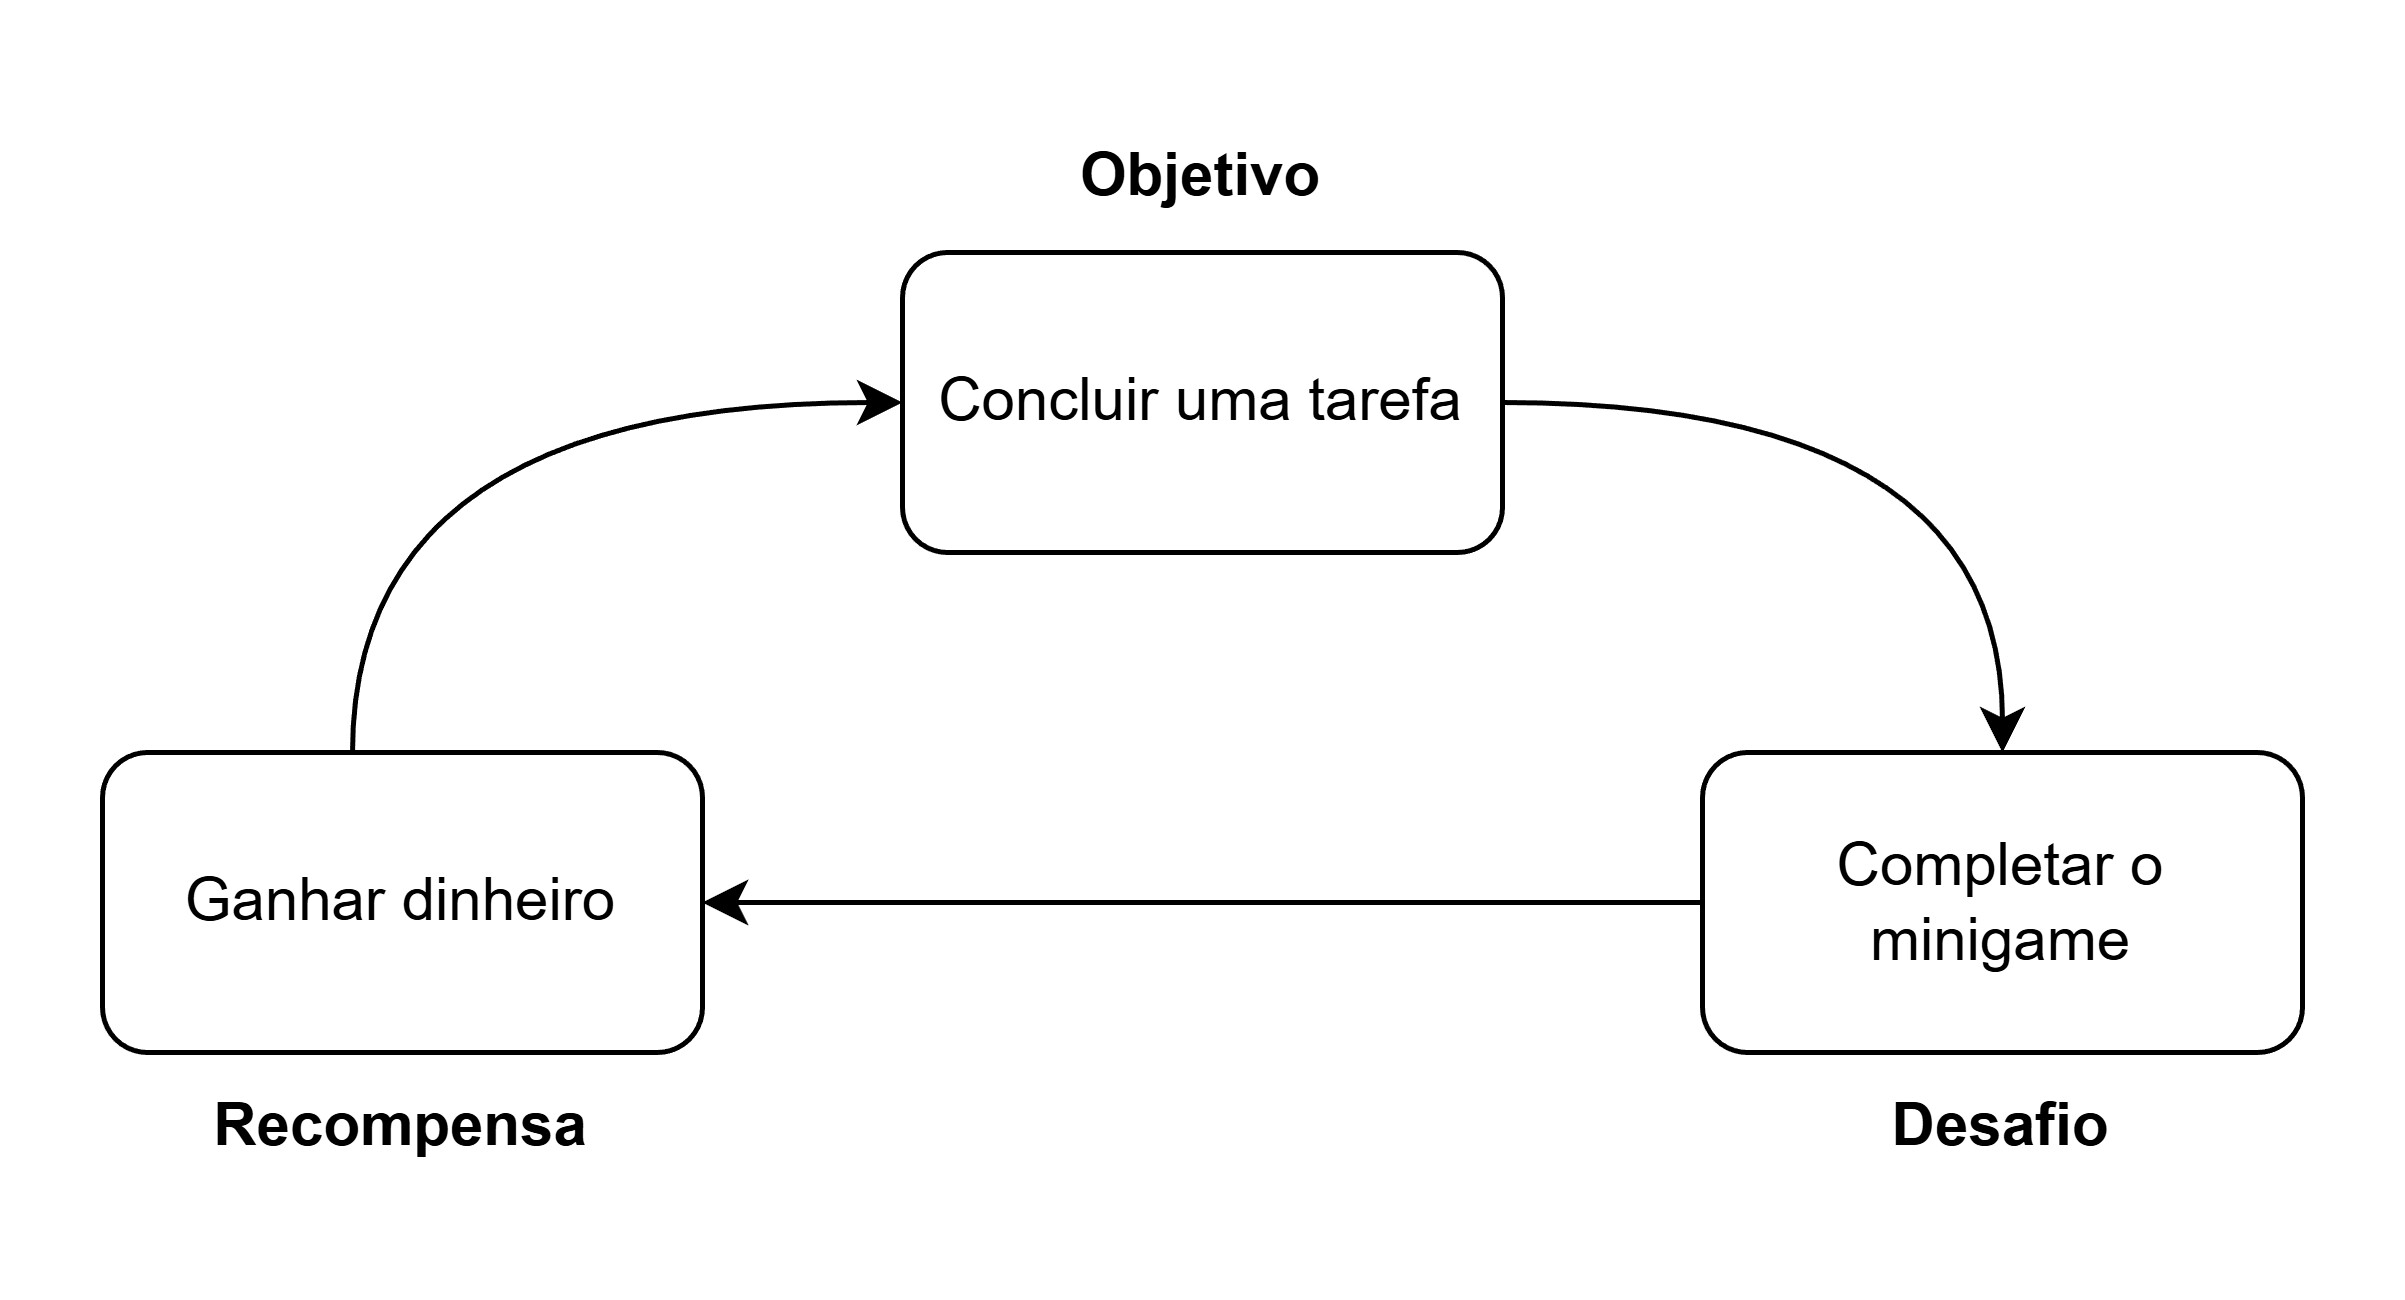
\includegraphics[width=0.9\textwidth]{Diagramas/Core_Gameplay_Loop.jpg}
    \caption{Diagrama do \textit{core gameplay loop} do jogo desenvolvido.}
    \label{Core_Gameplay_Loop}
\end{figure}

A Figura \ref{Core_Gameplay_Loop} apresenta o diagrama do \textit{core gameplay loop}, ou seja, o ciclo de ações principais do jogo.
A tarefa referida no diagrama, diz respeito aos pedidos dos clientes. Esses pedidos aparecem de forma constante e periódica durante toda a \textit{gameplay} além de representarem a principal forma do jogador conseguir dinheiro.

\newpage

A seguir apresenta-se os \textit{gameplay loops} secundários, ou seja, os ciclos de ações relacionados com a compra e configuração de equipamentos, e o ciclo de ações relacionado com o combate.

\begin{figure}[H]
    \centering
    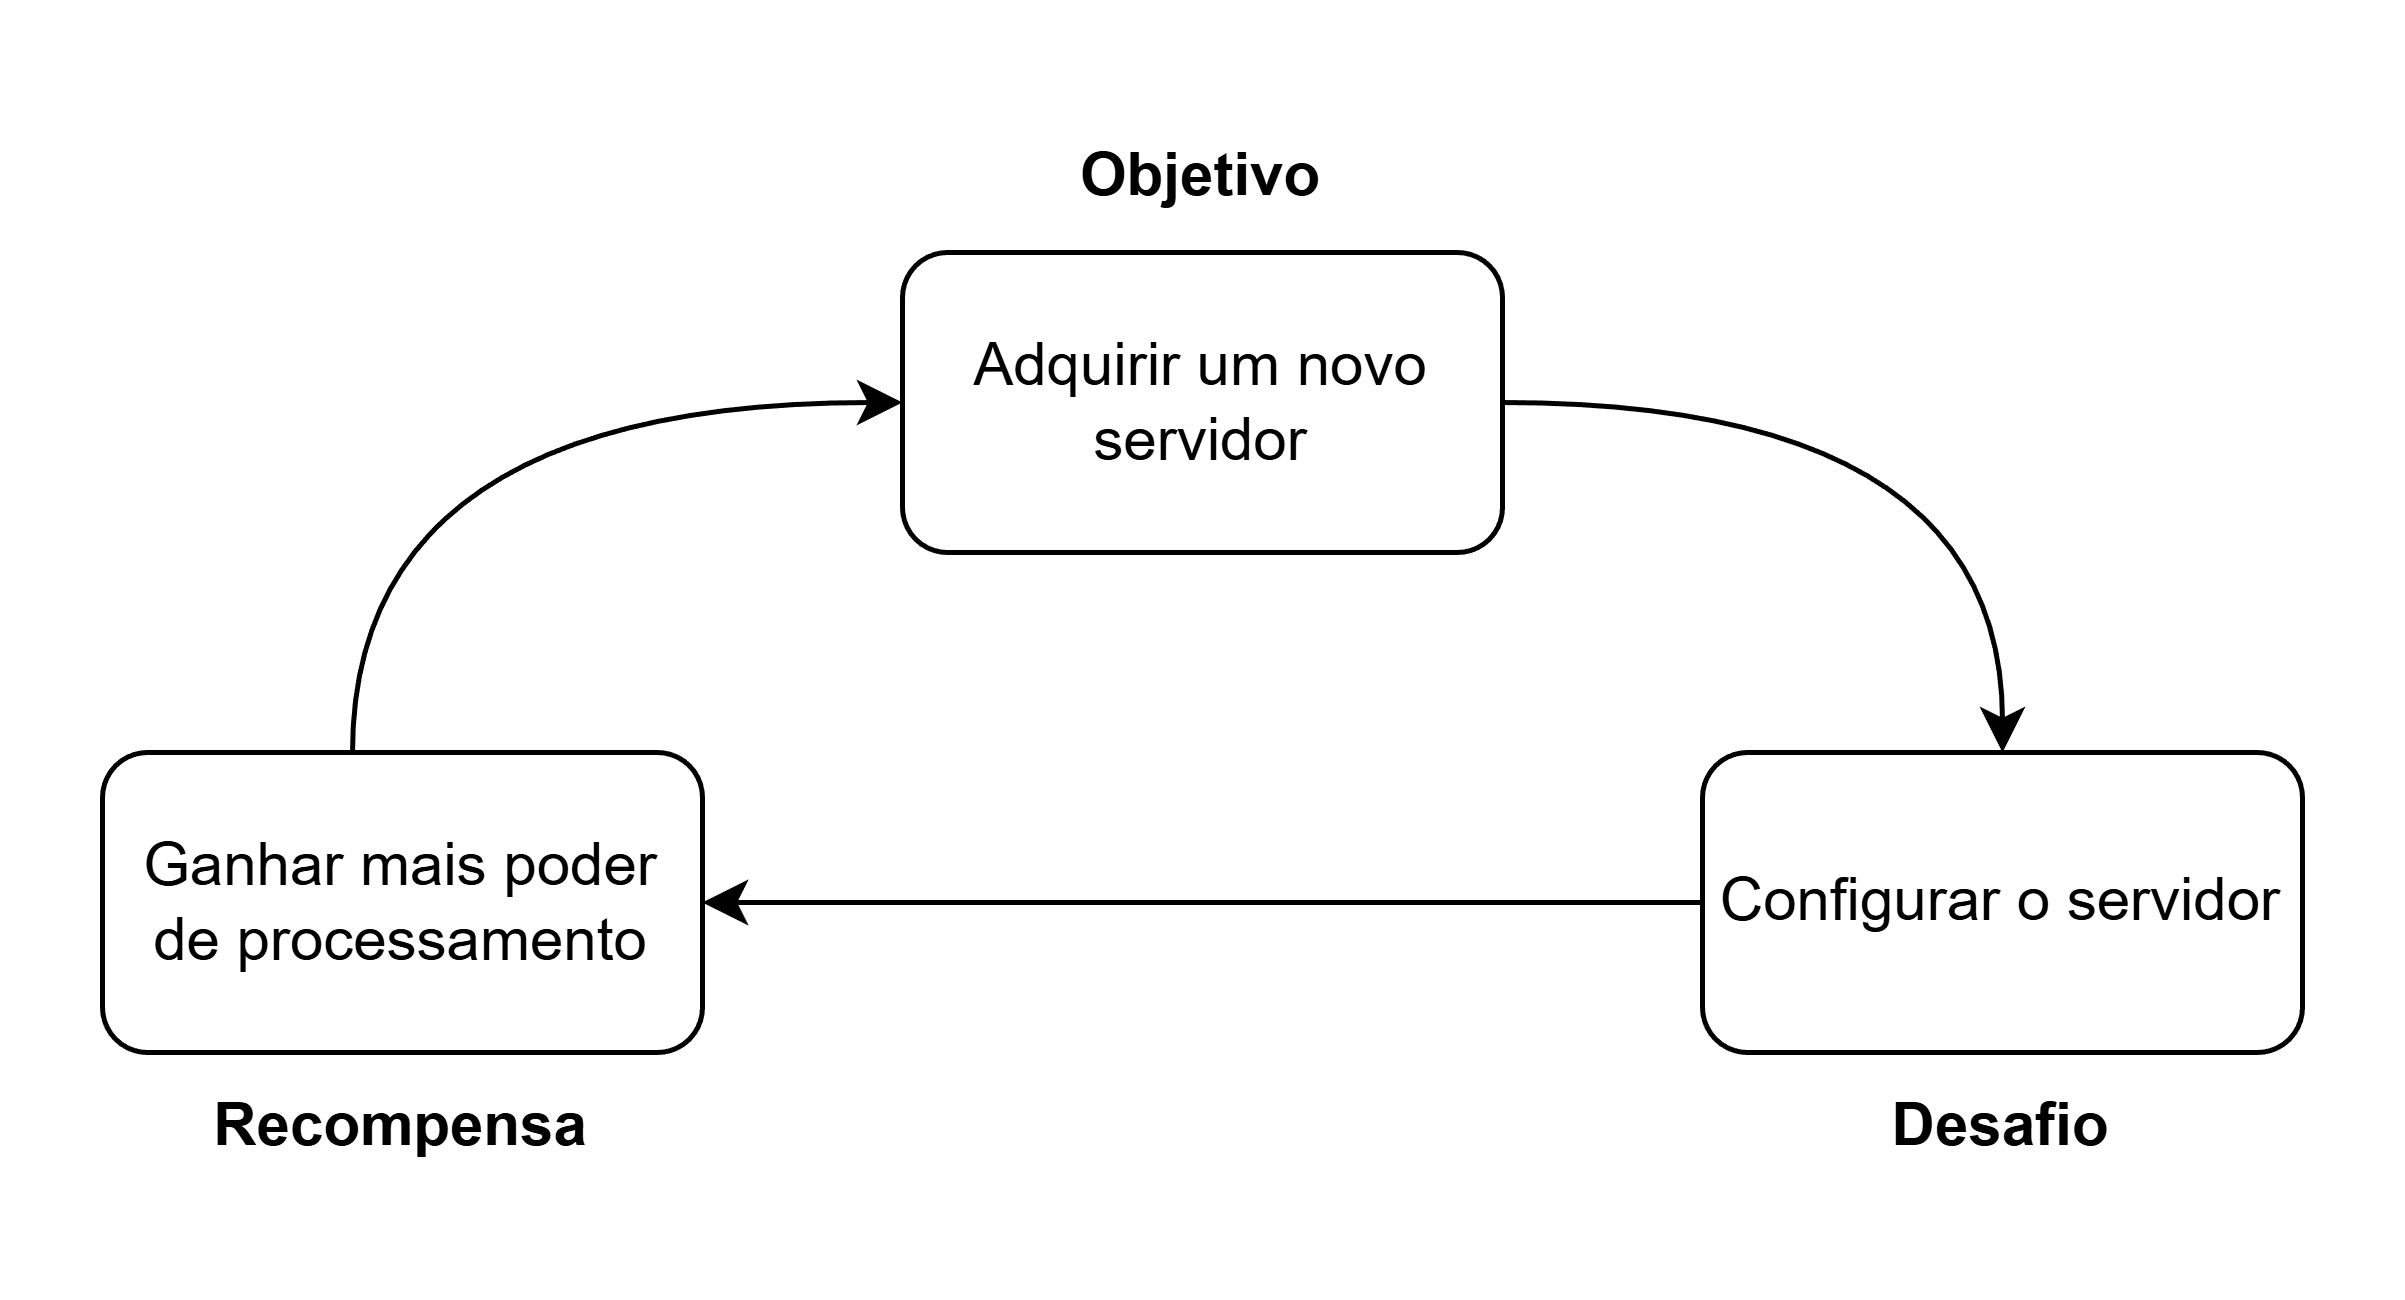
\includegraphics[width=0.9\textwidth]{Diagramas/Shop_Gameplay_Loop.png}
    \caption{Diagrama do \textit{gameplay loop} referente à configuração de servidores.}
    \label{Servers_Gameplay_Loop}
\end{figure}


\begin{figure}[H]
    \centering
    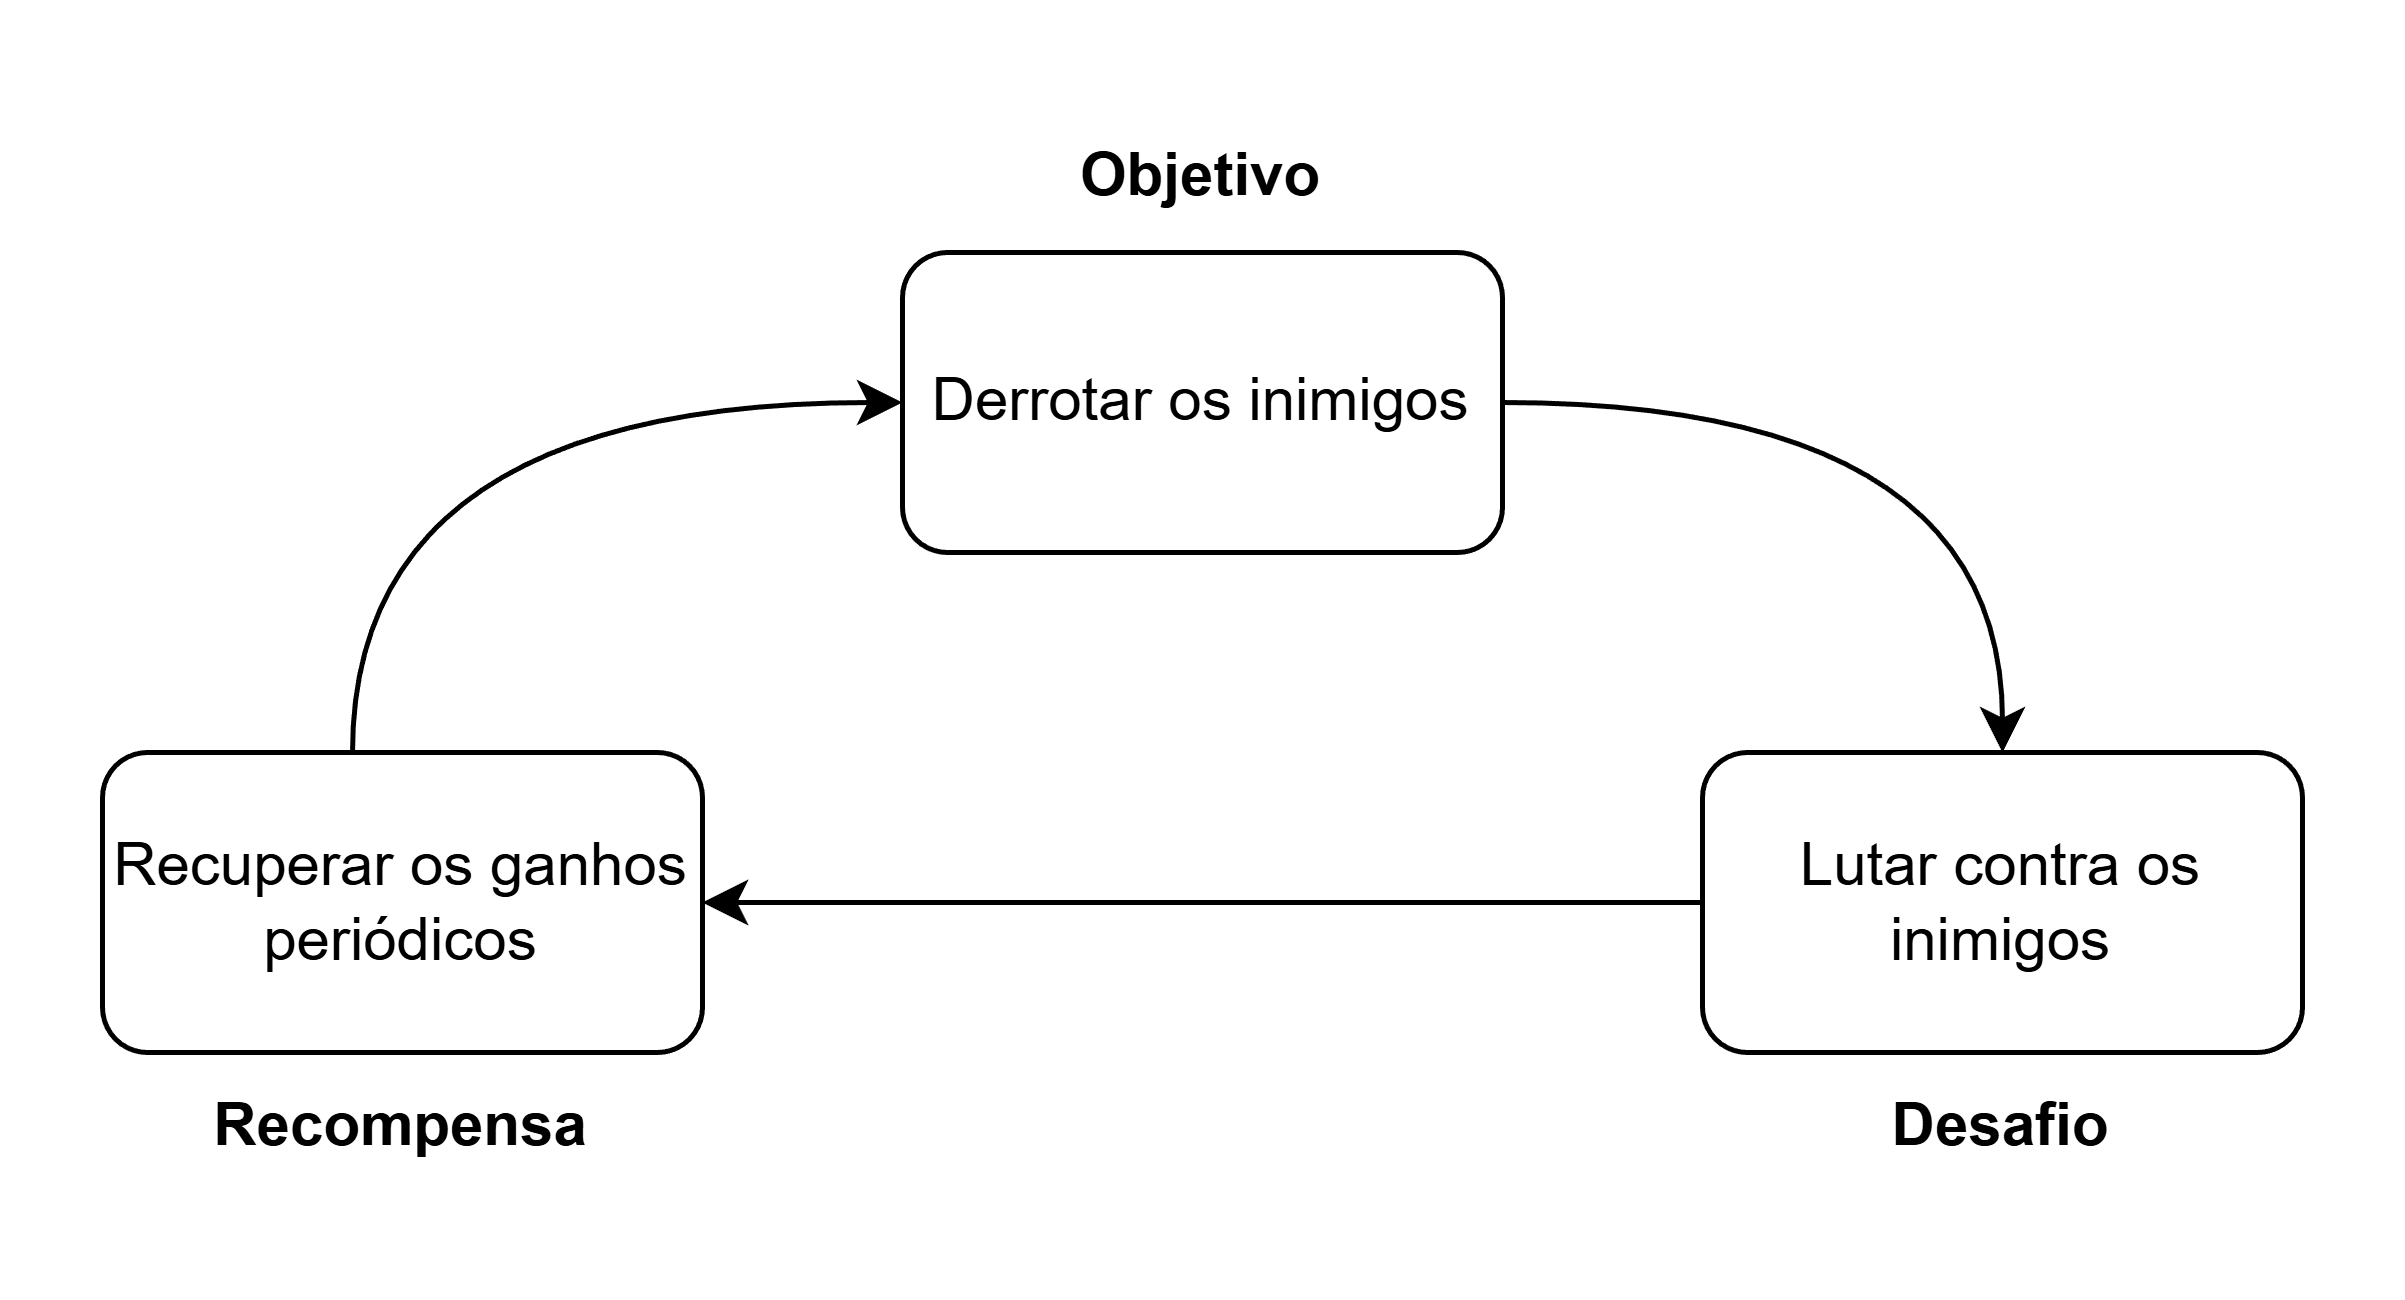
\includegraphics[width=0.9\textwidth]{Diagramas/Combat_Gameplay_Loop.png}
    \caption{Diagrama do \textit{gameplay loop} referente ao combate.}
    \label{Combat_Gameplay_Loop}
\end{figure}


